\chapter{Introduzione}\label{chp:Lamiere}
\section{Proprietà meccaniche sulla deformabilità}
Per un materiale metallico, le lavorazioni che si basano sulla deformazione del materiale sono:
\begin{itemize}
\item Forgiatura;
\item Laminazione;
\item Estrusione;
\item Trafilatura;
\end{itemize}
Di queste, le prime 3 provocano compressione nel materiale che, dunque, permettono al materiale metallico di mantenere le caratteristiche meccanico-fisiche. Essendo comunque compresso, il materiale risulta più duttile.
Per quanto riguarda invece la trafilatura, in questo caso si ha una trazione del materiale. Il che si traduce in una perdita di duttilità dovuta alla deformazione, prima elastica e poi plastica, del materiale. Ciò altera le proprietà meccanico-fisiche.
Tutto ciò è vero in particolare per lavorazioni massive: operazioni che vanno a modificare tutte e tre le dimensioni del materiale.
\newline
Se invece si prendono in considerazione le lamiere: prodotti di materiale metallico note per aver una delle tre dimensioni particolarmente ridotta, lo spessore nello specifico, la situazione cambia. Infatti non si può più considerare una qualsiasi deformazione in tutte e tre le dimensioni spaziali.
Inoltre, comprimendo una lamiera si rischia di piegarla. Dunque le lavorazioni su lamiera sono in genere, ma non sempre, per trazione.
Inoltre si vuole ricordare come la laminazione non sia una lavorazione su lamiera in quanto si ipotizza che la lamiera sia già laminata, dunque pronta a successivi trattamenti.
La maggior parte delle lavorazioni su lamiera vengono eseguite a freddo: ciò, come si vedrà in seguito, garantirà il mantenimento di determinate caratteristiche meccanico-fisiche.

\subsection{Tensione a freddo nelle lavorazioni a freddo}

\begin{figure}
\centering
\subfloat[][\emph{Grafico ingegneristico della prova di trazione}\label{fig:TrazioneContinua}]{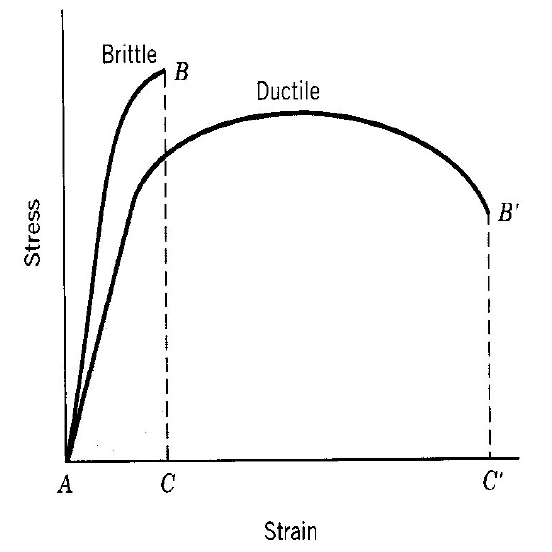
\includegraphics[width = 0.4\textwidth]{ProvaTrazione}} \quad
\subfloat[][\emph{Grafico prova di trazione con snervamento discontinuo}\label{fig:trazioneDiscontinua}]{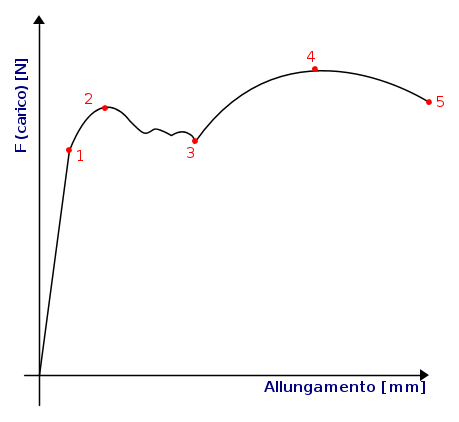
\includegraphics[width = 0.4\textwidth]{TrazioneDiscontinua}}
\caption{Prove di trazione}\label{fig:Trazione}
\end{figure}
Se si osserva il grafico della prova di trazione \ref{fig:TrazioneContinua}
si osservano 2 particolari zone: comportamento elastico del materiale e comportamento plastico.
Ricordando l'equazione constitutiva del materiale ovvero
\begin{equation}
\sigma = K \epsilon ^n
\label{eq:Cost}
\end{equation}
Dove i termini di \ref{eq:Cost} sono:\\
\begin{tabular}{cl}
$\sigma$ & tensione [MPa]\\
$K$ & coefficiente di resistenza\\
$\epsilon$ & fattore di incrudimento\\
$n$ & Sensibilità alla velocità di incrudimento\\
\end{tabular}
\\
Dalla \ref{eq:Cost} si può intuire che il il fattore $K$ lo si voglia particolarmente grande al fine di garantire un'alta resistenza allo snervamento.
La strizione si manifesterà su una sezione "più debole" (impurità, vuoti, ecc\dots), da cui avrà luogo una deformazione della sezione stessa. Dunque sulla sezione si manifesterà incrudimento dovuto proprio alla trasformazione.
L'incrudimento renderà la sezione molto più dura rispetto alle circostanti. Perciò si può dimostrare come il valore per cui la strizione si stabilizza è proprio pari al coefficiente $n$.
Sotto queste ipotesi allora vale:
\begin{equation}
\epsilon = n
\label{eq:StrizzCost}
\end{equation}
In generale si preferisce utilizzare materiali con coefficiente $n$ molto alto: per cui il materiale 
si deforma molto prima della strizione. Dunque è più \textbf{duttile}.

\subsection{Snervamento discontinuo}
Lo snervamento discontinuo è tipico dei metalli che hanno basso valore interstiziale.
Tipicamente, a fine lavorazione di tali metalli si presentano le \textbf{bande di Lüder}. Di fatto non costituiscono un difetto tecnologico, piuttosto puramente estetico. Siccome le lamiere vengono utilizzate anche per coperture, tali bande fanno sembrare il prodotto più scadente (Anche se di fatto non lo è).
Il grafico \ref{fig:trazioneDiscontinua} rappresenta il comportamento di un materiale a snervamento discontinuo.

\section{Tessitura e anisotropia}
La tessitura è la descrizione della presentazione, sia estetica che prestazionale, del materiale
Logicamente dipende direttamente dai grani cristallini presenti nel materiale.

Quando questi si presentano in forma allungata (es. post laminazione), portano 
a delle differenze dal punto di vista meccanico-fisico del prodotto. 
Portando \textbf{anisotropia}.
Già si sa che i piani preferenziali di scorrimento sono quelli ad alte densità atomica
e, nel caso non ce ne siano a sufficienza, il materiale tenderà a costituirne di nuovi%
\footnote{Si vedrà anche in seguito che la questione dei piani di scorrimento è cruciale per la qualità del materiale}.

\subsection{Proprietà modificate}
Ricordando i principali termini di descrizione delle proprietà meccanico-fisiche dei metalli:\\
\begin{tabular}{cl}
$Y$ & Densità di snervamento\\
$T_S$& Resistenza meccanica\\
\end{tabular}
\\
Inoltre anche altre proprietà, non necessariamente meccaniche, vengono modificate da eventuali lavorazioni a freddo.
Allora: considerando una lamiera lavorata a freddo vale:
\begin{equation}
\epsilon_1 + \epsilon_2 + \epsilon_3 = 0 \underbrace{\rightarrow}_{\text{per lamiere}}
\epsilon_l + \epsilon_w + \epsilon_t = 0 
\label{eqn:DefCost}
\end{equation}
La \ref{eqn:DefCost} definisce la \emph{costanza della deformazione del volume principale}.
Si considerano pedici diversi da quelli classici per un volume massivo in quanto stiamo considerando una lamiera, per cui i nuovi pedici indicano:\\
\begin{tabular}{cl}
$l$ & \textit{lenght}\\
$w$ & \textit{width}\\
$t$ & \textit{thickness}\\
\end{tabular}
\\
Si ricordano, inoltre, le deformazioni per le principali grandezze:
\begin{equation}
\epsilon_w = \ln{\frac{w_1}{w_0}} \qquad \epsilon_t = \ln{\frac{h_1}{h_0}}
\label{eqn:DefPrinc}
\end{equation}
Dove $w_1$ e $h_1$ sono le misurazioni dopo la prova di trazione, mentre $w_0$ e $h_0$ sono i valori iniziali.
A partire dai termini sopraelencati, si può definire il parametro $r$ definito come nella \ref{eqn:r}.
\begin{equation}
r = \frac{\epsilon_w}{\epsilon_t}
\label{eqn:r}
\end{equation}
Non ha un nome specifico, nonostante rappresenti la quantità di deformazione che una lamiera subisce se sottoposta a trazione.
In particolare, le due deformazioni considerate sono quella in termini di spessore e quella in larghezza.
Se il materiale avesse:
\begin{equation}
r = 1
\end{equation}
potrebbe essere considerato isotropo. Più correttamente si definiscono \textbf{isotropi} tutti quei materiali per cui vale la \ref{eqn:DefIsotropo}.
\begin{equation}
r_0 = r_{45} = r_{90} = 1
\label{eqn:DefIsotropo}
\end{equation}
dove i fattori $r$ sono il rapporto tra le deformazioni come sopra però ponendo la trazione con angolo tanto quando indicato dal pedice:\\
\begin{tabular}{cl}
$r_0$ & Direzione laminazione\\
$r_{45}$ & Direzione intermedia\\
$r_{90}$ & Direzione ortogonale
\end{tabular}
\\
Altrimenti il materiale è semplicemente \textbf{anisotropo}.
L'anisotropia può essere un problema in termini di lavorazione di una lamiera: si prenda come esempio il caso della realizzazione di un contenitore per estrusione. Se il materiale fosse isotropo allora la deformazione avverrebbe in maniera uniforme su tutta la lamiera.
Se, invece, il materiale è anisotropo, la deformazione diversificata produce variabilità sul bordo del prodotto. Successivamente sarebbe necessario un operazione di \textit{trimming} per eliminare il materiale in eccesso.
L'anisotropia si può verificare in diverse forme.
\begin{description}
\item[$r_0 = r_{45} = r_{90} \lessgtr 1$] allora si parla di \textbf{Anisotropia normale} alla superficie della lamiera. Se ne può misurare il valore tramite:
\begin{equation}
r_m = \overline{r} = \frac{r_0 + r_{90} + 2 * r_{45}}{4}
\label{eqn:MisAnisotropia}
\end{equation}
\item[$r_0 \neq r_{45} \neq r_{90}$] allora si parla di \textbf{compresenza di anisotropia planare e normale} da cui si può ottenere una misura
\begin{equation}
\Delta r = \frac{r_0 + r_{90} - 2 * r_{45}}{2}
\label{eqn:MisPlanare}
\end{equation}
\end{description}
In generale l'anisotropia si verifica quando, durante la laminazione, i reticoli cristallini si muovono per garantire i piani di scorrimento.
Ora si vuole dare una rapida visione delle principale strutture cristallini nei materiali.

\subsubsection{Reticolo esagonale compatto}
I piani di scorrimento si trovano sulle superfici di base del prisma compatto.
Si definisce \textit{compatto} perché il rapporto tra l'altezza del prisma e la lunghezza di un lato di base, ovvero $c/a$ considerando i riferimenti della figura \ref{fig:EsaComp}.
\begin{figure}
\centering
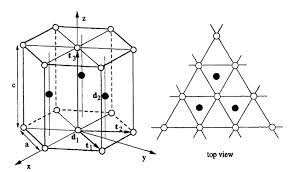
\includegraphics[width = 0.8\textwidth]{Esagono1}
\caption{Esagonale compatto}
\label{fig:EsaComp}
\end{figure}
Si osserva che il rapporto \ref{eqn:r} per materiali con reticolo cristallino \eng{High c/}a è prossimo a a 0:
\begin{equation}
r_{\text{High c/a}} = \frac{\epsilon_w}{\epsilon_t} \longrightarrow 0
\label{eqn:HighC_AR}
\end{equation}
Nella maggior parte dei casi si vuole un rapporto $r$ il più alto possibile. Così ché la deformazione della lamiera interessi la larghezza piuttosto dello spessore. Altrimenti potrebbero sorgere problemi sulla rigidità della lamiera anche senza eseguire alcuna lavorazione.
Potremmo allora dire che:
\begin{description}
\item[$n$] indichi il ritardo nella deformazione (sensibilità alla deformazione)
\item[$r$] indichi che tipo di deformazione si avrà. 
\end{description} 

Nel caso di materiali ad esagonale compatto ma con rapporto $c/a$ basso si osserva:
\begin{equation}
r_{\text{Low c/a}} \longrightarrow \infty 
\end{equation}
Ad esempio per guadagnare duttilità nel titanio (Ti) si effettuano lavorazioni a caldo.

\subsubsection{Reticolo cubico}
\begin{figure}
\centering
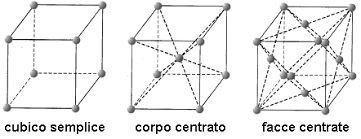
\includegraphics[width = \textwidth]{Cubico}
\caption{Reticoli cubici}
\label{fig:Cubici}
\end{figure}
Per i metalli cristallizzanti a \ac{CFC} si osserva un valore di $r\approx 0.4 \div 0.8$.
Mentre per i metalli a \ac{CCC} si osservano valori di $r \approx 1$.

\section{Effetti delle lavorazioni a freddo}
Come già accennato in precedenza, le lavorazioni a freddo permettono di ottenere da un materiale metallico sì la deformazione voluta. In più si garantisce al materiale maggiore durezza.
Ciò è dovuto allo scorrimento delle dislocazioni, durante la lavorazione del materiale, che vengono bloccate dal bordo del grano cristallino.
Di contro bisogna tenere a mente che una maggiore durezza impone una minore duttilità, considerazione che serve nel caso la lamiere debba subire diverse lavorazioni prima di divenire prodotto finito.

Dunque le lavorazioni a freddo hanno diversi vantaggi e svantaggi come descritto nella tabella \ref{tab:VantSvantFreddo}.

\begin{table}
\centering
\caption{Vantaggi e svantaggi delle lavorazioni a freddo}
\label{tab:VantSvantFreddo}
\begin{tabularx}{\textwidth}{XX}
\toprule
\textcolor{UnifeDark}{\textbf{Vantaggi}} & \textcolor{UnifeDark}{\textbf{Svantaggi}}\\
\midrule
Metodo economico per indurire il materiale &
Pressione sugli stampi più alti\\
Il prodotto è quasi finito finite le lavorazioni (in genere) &
Bisogna trovare un compromesso tra durezza desiderata e consumo delle attrezzature\\
\bottomrule
\end{tabularx}
\end{table}

Per ovviare ad alcuni problemi evidenziati alla tabella \ref{tab:VantSvantFreddo}, si può pensare di ricorrere a ricotture parziali o complete.
Alcuni esempi sono riportati alle figure \ref{fig:RsRicottura}

In particolare:
\begin{description}
\item[Lavorazione a freddo $T < 0.3 T_m$] evidenzia un chiaro incrudimento del materiale, che ne risulterà indurito.
\item[Ricotture di distensione $0.3T_m < T < 0.5 T_m$] Permette una ridistribuzione delle dislocazioni ma senza ricristallizzazione
\item[Ricottura di ricristallizzazione $T > 0.5 T_m$] Non è scontata la ricristallizzazione ma si ha una distensione dei grani, annullando eventuali lavorazioni a freddo precedenti.
\end{description}
Nonostante ciò le ricotture possono essere molto interessanti per le caratteristiche meccaniche dei materiali metallici.
Ipotizzando di voler raggiungere un determinato obbiettivo di duttilità del materiale. Si può raggiungere tale obbiettivo semplicemente lavorando il materiale a freddo, dando una certa deformazione al pezzo.
Sappiamo che così il pezzo sarà più indurito di conseguenza.
C'è un ulteriore modo: se si incrudisce di più rispetto al obbiettivo, attraverso una deformazione maggiore di quella desiderata, si può pensare di sfruttare una ricottura di distensione per ritornare al livello di duttilità richiesto ma garantendo un livello di durezza maggiore rispetto alla sola lavorazione a freddo. In genere vale anche il viceversa. 
Tale metodo viene chiamato \textit{forte incrudimento con ricottura parziale}.
Alla figura \ref{fig:Ricot} è graficato l'andamento delle tensioni di snervamento e rottura dopo una ricottura completa. Si osserva che vengono perse completamente le caratteristiche meccaniche guadagnate tramite incrudimento per lavorazione a freddo.
Alla figura \ref{fig:RicotRs} viene mostrato il processo per ottenere una determinata tensione di snervamento dopo forte incrudimento. 

\begin{figure}
\centering
\subfloat[][\emph{Duttilità, snervamento e rottura dopo ricottura}\label{fig:Ricot}]%
{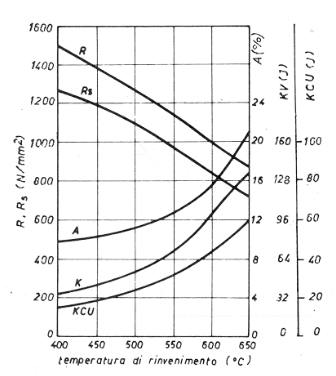
\includegraphics[width = 0.4\textwidth]{Rinvenimento}}\quad
\subfloat[][\emph{Durata ricottura in base allo snervamento richiesto}\label{fig:RicotRs}]%
{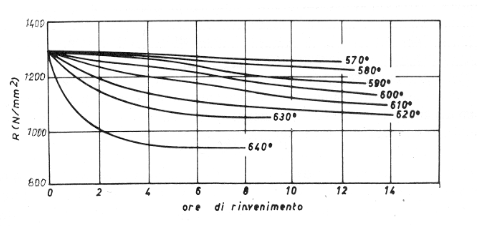
\includegraphics[width = 0.4\textwidth]{CotturaRinvenimento}}
\caption{Andamenti tipici di un acciaio dopo ricottura}\label{fig:RsRicottura}
\end{figure}

Ipotizzando una ricottura completa, ovvero portando il materiale a una temperatura $T > 0.5\:T_m$, si può avere ricristallizzazione del metallo che porta grani a dimensioni maggiori. Bisogna anche tenere a mente l'influenza del tempo su questi processi di ricottura.

\subsection{Effetti della velocità di deformazione}
Come visto nell'equazione costitutiva \ref{eqn:DefCost}, il materiale viene univocamente definito tramite tale equazione. In realtà è necessario "mettere in relazione" anche il tempo. Considerando l'equazione costitutiva per lavorazione a caldo:
\begin{equation}
\sigma_f = C \cdot \dot{\epsilon}^m
\label{eqn:CostCaldo}
\end{equation}
Da cui si può osservare che se la temperatura aumenta allora $C$ diminuisce e contemporaneamente $m$ cresce. Infatti:
\begin{description}
\item[$C$] è il coefficiente di resistenza alla temperatura del materiale;
\item[$m$] è l'indice di sensibilità alla velocità di deformazione;
\item[$\dot{\epsilon}$] è la velocità di deformazione descritta come $V/h$
\end{description}
Con una strizione diffusa, l'incrudimento è diffuso su tutto il provino. E, come si era visto anche in precedenza, ciò migliora le caratteristiche meccaniche. Se invece, la strizione è localizzata rischia di indebolire il materiale.
Il fatto che sia locale indica che il materiale in quel punto è più debole e può rompersi più facilmente.

\begin{definition}{Considerazione}{*}
In generale si privilegiano metalli che abbiano alta sensibilità al incrudimento e maggiore sensibilità alla velocità di strizionamento.
\end{definition}


Si vogliono ricordare i valori per cui $m$ porta ad un determinato comportamento il materiale:
\begin{description}
\item[$-0.05 < m < 0.05$] \eng{Cold working}
\item[$0.05 < m < 0.3$] \eng{Hot working}
\item[$0.3 < m < 0.7$] \eng{Superplasicity}%
\footnote{Valori di deformazione tipici delle lavorazioni con materiali plastici}
\item[$m > 1$] \eng{Newtonian fluid}
\end{description}

\section{Limiti di formabilità delle lamiere}
\begin{enumerate}
\item Manifestazione di strizioni localizzate.
\item Con strizione diffusa, prima della rottura.
\item Generazione delle bande di Lüders
\item Generazione della superficie a buccia d'arancia
\end{enumerate}
A parte le prime due che portano a conseguenze meccaniche per cui la lamiera effettivamente non può più essere vendute o utilizzate per la produzione.
La terza ha una motivazione puramente estetica: siccome le lamiere possono essere utilizzate come copertura, tale superficie può essere problematica. Non lo è dal punto di vista meccanico-fisico.
La superficie a buccia d'arancia anch'essa non influisce sulle prestazione meccaniche del prodotto%
\footnote{C'è da dire che una maggiore porosità superficiale potrebbe stimolare la generazione di cricche in alcune lavorazioni.}.
La formazione è dovuta alla rotazione dei grani cristallini durante eventuali lavorazioni.
La soluzione è quella di sfruttare, per le lamiere in particolare, materiali a grana fine.

\subsection{Come mai le lamiere?}
Le lamiere vengono largamente impiegate per la produzione di oggetti metallici, e le tecniche che verranno trattate in questo corso volgono a a sfruttare tale prodotti in larga scala.
Alcuni motivi dell'espansione del loro impiego sono:
\begin{itemize}
\item A parità di prodotto, un oggetto pieno e uno ricavato tramite lavorazione di lamiera risulta più pesante.
\item La laminazione è una lavorazione molto efficiente: si producono tanti pezzi in poco tempo e con minore energia.
\item La laminazione permette di raggiungere risultati molto accurati (in termini di spessori e qualità del laminato) con poche risorse, dunque ad un costo molto basso.
\item La lamiera è un prodotto "quasi" pronto all'uso.
\end{itemize}

\section{Materiali per lamiere}
I materiali che in industria vengono più comunemente utilizzati per lamiere sono ad esempio:
\begin{itemize}
\item Acciai, dolci + inossidabili
\item Leghe di allumino
\item Ottoni
\item Bronzi
\item Rame
\item Magnesio
\item Titanio
\end{itemize}
Sebbene la maggior parte dei prodotti in lamiera siano lavorati a freddo, ci sono alcuni materiali che necessitano di lavorazioni a caldo.
In particolare alla figura \ref{fig:LavCaldo}, si presentano i motivi per cui sia necessaria la lavorazione a caldo

\begin{figure}
\centering
\usetikzlibrary{trees}
\begin{tikzpicture}[
sibling distance = 10em,
every node/.style={rectangle, rounded corners, draw, align=center}]
\node[top color=UnifeLight]{Lavorazioni a caldo}
	child{node[top color=UnifeDark, bottom color=UnifeDark!50, white]{Esagonale\\compatto}
		child{node[top color=UnifeDark!50, bottom color=UnifeDark!50, white]{Maggiore\\duttilità}}
		child{node[top color=UnifeDark!50, bottom color=UnifeDark!50, white]{Si spera in\\un cambio\\di reticolo}}}
	child{node[top color=UnifeDark, bottom color=UnifeDark!50, white]{Superplasticità}}
	child{node[top color=UnifeDark, bottom color=UnifeDark!50, white]{Forze troppo\\alte}};
\end{tikzpicture}
\caption{Motivazioni delle lavorazioni a caldo}
\label{fig:LavCaldo}
\end{figure}
Ora si vedranno nel dettaglio tutte le caratteristiche e motivazioni per cui viene scelta una determinata categoria di materiali.

\subsection{Acciai}
In genere si preferiscono acciai che abbiano un tenore di carbonio minore del 0.15\%, ovvero gli acciai dolci.
Inoltre, bisogna includere gli acciai inossidabili: sia per motivi di mercato, che necessità operative dei prodotti finali.
Essendo una gamma decisamente ampia di materiali, le lavorazioni possibili sono molteplici:
\begin{description}
\item[lavorazioni a caldo] non vengono sfruttate troppo per gli acciai in quanto si preferisce mantenere l'incrudimento ottenuto tramite la lavorazione a freddo. Anche se si impiega per:
	\begin{itemize}
	\item Ottenere maggiore duttilità per il materiale.
	\item Quando le forze in gioco sono eccessive è opportuno aumentare la duttilità grazie ad 
	una maggiore temperatura.
	\end{itemize}
	Si rischia di incorrere in:
	\begin{itemize}
	\item Finiture peggiori.
	\item Maggiore rugosità da cui derivano pure caratteristiche meccaniche peggiori.
	\item Non si ottiene incrudimento. 
	\end{itemize}
\item[Lavorazioni a freddo] In industria vengono sfruttate molto più volentieri per via:
	\begin{itemize}
	\item Migliori tolleranze geometriche ottenibili.
	\item Migliore finitura superficiale,
	\item Migliori prestazioni meccaniche a parità mi materiale usato.
	\end{itemize}
\end{description}

Si vuole approfondire anche gli aspetti legati alla tipologia degli acciai:
\begin{description}
\item[Acciai effervescente] Questi acciai presentano delle bolle di ossigeno (o comunque ossidi) all'interno, da qui il nome effervescente, dovute alla presenza del gas durante la colata.
\item[Acciai calmati] Sono acciai che vengono calmati tramite un processo di deossidazione in colata. Il processo viene realizzato tramite inclusione di alluminio e manganese per legare l'ossigeno e portarlo in superficie tramite una schiuma separabile dal fuso.
\end{description}

Per gli acciai è significativa la formazione delle famose \textbf{bande di Lüders}.
Possono eventualmente essere eliminate tramite un processo di \eng{skin-pass}, ovvero un processo di laminazione a bassa deformazione che permette di eliminare lo snervamento discontinuo.
Purtroppo non è permanente: l'invecchiamento del materiale porta si l'eliminazione della discontinuità ma allo stesso tempo incrudisce il materiale che diventa più duro che duttile.
In genere, dopo il trattamento di \eng{skin-pass} la lamiera trattata deve essere utilizzata in tempi molto brevi.
Altrimenti, sarà necessaria una laminazione più pesante che peggiora la duttilità.

\subsubsection{Acciai a basso tenori di carbonio}
Sono in assoluto i più usati tra i prodotti lamierati. Il tenore di carbonio si attesta attorno il $0.15\%$.

\subsubsection{Acciai effervescenti}
L'elevata duttilità e il costo relativamente basso hanno reso gli acciai effervescenti di qualità commerciale e adatti all'imbutitura.
Solo per applicazioni non critiche.
La superficie povera di carbonio è particolarmente adatta per processi di smaltatura.
La dimensione del grano è controllata con pesanti passate di laminazione a freddo fino al $50 \div 70 \%$ seguita da ricottura. 
Tuttavia la presenza di carbonio e azoto produce un allungamento del punto di snervamento e bande di Lüders. Come visto precedenza può essere risolto parzialmente in precedenza.

\subsubsection{Acciai calmati}
L'acciaio di qualità per trafilatura ha proprietà uniformi ed elevati valori di $n$. sensibilità all'incrudimento $r$, parametro usato per definire l'anisotropia che viene scelto quando si devono realizzare pesanti imbutiture o \eng{stretching} o quando l'immagazzinaggio è inevitabile.
Anche l'acciaio calmato contiene carbonio e azoto, ma quest'ultimo viene combinato con l'alluminio in un composto e solo il carbonio rimane in una forma che ne permetta la concentrazione presso le dislocazioni a formare le atmosfere di \eng{Cottrell}.
Anche le lamiere ricotte mostrano l'allungamento del punto di snervamento, ma lo \eng{skin-pass} elimina definitivamente l'allungamento in corrispondenza dello snervamento. Il carbonio non si diffonde ai siti delle dislocazioni a meno che l'acciaio non sia riscaldato ai $120\unit{\celsius}$.

\subsubsection{Acciai interstitial-free}
Il contenuto di carbonio è ridotto a livelli molto bassi e l'azoto è legato in piccole quantità di altri elementi. Non esiste un allungamento in corrispondenza dello snervamento, la tensione di snervamento è bassa, perciò è piccolo il ritorno elastico, e il valore di $n$ è elevato.

Nel settore automobilistico si cerca di ridurre il peso. La carrozzeria più sottile deve essere bilanciata da una resistenza maggiore, per cui la ricerca di un peso ridotto ha determinato lo sviluppo di materiali più resistenti. Tutti i meccanismi di rafforzamento sono utilizzati per questo scopo.

\subsubsection{Acciai ad alta resistenza}
Sono acciai che vengono già incruditi prima della lavorazione. 
Le tecniche di incrudimento possono essere:
\begin{itemize}
\item laminazione a freddo, può provocare delle piccole deformazione per cui in genere succedono delle ricotture di distensione, per riottenere una duttilità maggiore con una resistenza ragionevole. Oppure una ricottura completa per controllare la dimensione del grano.
\item precipitazione di soluzione solida, sono acciai che presentano in lega elementi come Mn, P, o Si  che incrudiscono più rapidamente.
\item incrudimento tramite ricottura, questi acciai sono laminati per eliminare le bande di Lüders. Dopo invecchiano rapidamente durante la verniciatura in forno. Determina un incremento della resistenza di circa $30 \div 40\unit{\MPa}$ grazie alla formazione di aree dense di C.
L'incremento di resistenza nell'invecchiamento può essere massimizzato aumentando il contenuto di N.
\end{itemize}

\subsubsection{Acciai Dual-phase}
Presentano tenore di C più alto, necessario per il trattamento di bonifica, è utile negli acciai per molle ma ridurrebbe troppo la duttilità negli acciai per imbutitura. Tuttavia acciai a basso tenore di carbonio con $1.4\%$ di Mn possono essere ricotti per ottenere una struttura costituita da ferrite rinforzata da martensite dispersa.
Questi acciai \eng{Dual-Phase} hanno una tensione di snervamento bassa che è un vantaggio quandop il ritorno elastico può essere contestato, nello stesso tempo, il rapido incrudimento durante le lavorazioni impartisce una resistenza elevata nel prodotto finale.

\subsubsection{Acciai HSLA}
L'uso di questi acciai aumenta progressivamente nelle automobili e in altre strutture. Una caratteristica negativa importante è il valore elevato del rapporto tra tensione di snervamento e modulo elastico che determina uno \eng{springback} elevato.

Inoltre è possibile che la laminazione permetta di zincare o stagnare le lamiere.
Zincatura permette maggiorata resistenza alla corrosione, ma può essere problematica in funzione del tenore di carbonio, e latri elementi in lega. Garantisce maggiorata resistenza alla corrosione atmosferica anche in caso di graffi e abrasioni.
La stagnatura permette di migliorare la resistenza alla corrosione ma è sensibile a ripetuti graffi, per cui può essere problematica.

La laminazione permetterebbe anche altri tipi di rivestimenti, come verniciature in foglio ecc\dots

\subsubsection{Acciai inossidabili}
Presentano alte capacità di incrudimento, dunque la loro formabilità è eccellente.
I più utilizzati sono sicuramente gli inox austenitici: garantiscono la migliore resistenza alla corrosione con ottima formabilità per via della matrice austenitica.
Il campo di applicazione più adatto è sicuramente legato all'alimentare: posate, pentole ecc\dots
Siccome presentano alte deformabilità, si realizzano anche lavelli, scambiatori di calore e diverse apparecchiature per processi chimici.

Gli acciai inossidabili martensitici e ferritici si possono impiegare nei casi in cui non sono necessarie resistenza alla corrosione così spinte e formabilità limitata.
Sicuramente hanno un costo inferiore.

\subsection{Metalli non ferrosi}
Altri materiali, che non sono leghe a base di ferro, vengono abitualmente impiegati nella produzione di oggetti laminati.

\subsubsection{Rame e ottoni}
Il rame, in diverse leghe tra cui gli ottoni, sono tra i materiali più deformabili in assoluto. Vengono abitualmente utilizzati.

\subsubsection{Alluminio}
Le leghe di alluminio, possono essere utilizzate per deformazione a freddo,alcune possono presentare degli snervamenti seghettati (Serie 5000) che porta a dei segni superficiali contestabili. Leghe indurite per precipitazione non presentano questo problema (Serie 6000).
Possono essere migliorate tramite \ac{TT} che migliora significativamente il rafforzamento. 
Ulteriore processo di rafforzamento è dato dal processo di invecchiamento T4 che può essere imposto alle leghe di alluminio.

Per molte applicazioni la rugosità superficiale può essere critica.
IN alcuni casi si preferisce una rugosità maggiore, ovviamente controllata, per favorire l'adesione della vernice. Resta il fatto che asperità troppo pronunciate si vedano anche a processo completato. In più, una superficie poco porosa non tratterrebbe il lubrificante nel contatto lamiera stampo. Per cui si potrebbero avere delle situazioni di saldatura a freddo tra lamiera e stampo.

Tuttavia, la rugosità spinta non permetterebbe una buona distribuzione della pressione di stampaggio e non può essere controllato il flusso di metallo nello stampo.
Un orientamento casuale delle caratteristiche superficiali è preferibile per migliorare l'aspetto ed è essenziale per assicurare un allungamento uguale in tutte le direzioni.

La rugosità tipica è di $R_a = 1 \div 1.5\unit{\um}$.
La tecnica più diffusa per la realizzazione di tale finitura superficiale è la laminazione con rulli pallianti in modo casuale.
Più recentemente, i rulli hanno una tessitura superficiale: crateri formati in modo predeterminato medianti raggi laser o scariche elettriche.


\chapter{Lavorazioni su lamiera}\label{chp:Lavlamiera}
La figura \ref{fig:LavLamiera} presenta le possibili lavorazioni su lamiera.
Si possono includere in queste lavorazioni anche fili, profilati e tubi.

\begin{figure}
\centering
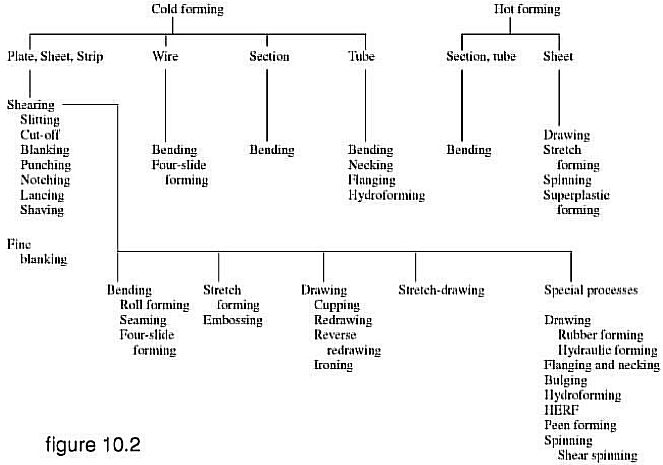
\includegraphics[width = \textwidth]{LavLamiera}
\caption{Possibili lavorazioni su lamiera}
\label{fig:LavLamiera}
\end{figure}

In generale la sequenza delle lavorazioni per prodotti in lamiera è:
\begin{enumerate}
\item taglio,
\item deformazione plastica,
\item giunzione.
\end{enumerate}
Ovviamente la sequenza non è ferrea, dipende dal ciclo produttivo necessario al prodotto. Sicuramente la maggior parte dei prodotti segue questa prima sequenza.

Dunque come prima lavorazione su lamiera si parlerà del taglio.

\section{Taglio di lamiera}
In figura \ref{fig:TaglLamiera} sono riportati alcuni esempi di operazioni di taglio su lamiere, nastri, fili ecc\dots

\begin{figure}
\centering
\subfloat[][\emph{Possibili tagli su lamiere e affini}\label{fig:TaglLamiera}]
{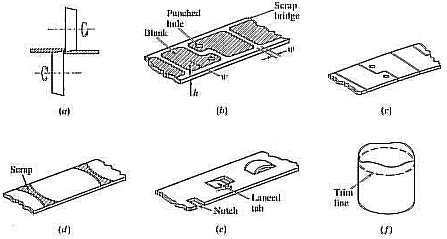
\includegraphics[width = 0.4\textwidth]{TaglLamiera}}\quad
\subfloat[][\emph{Differenza tra punzonatura e tranciatura}\label{fig:TaglLamiere2}]
{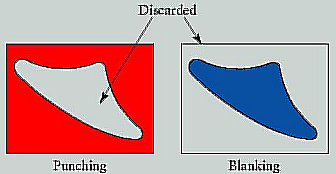
\includegraphics[width = 0.4\textwidth]{TaglLamiera2}}
\caption{Operazioni di taglio su lamiere e affini}
\label{fig:TaglLam}
\end{figure}

Il primo passo, indipendentemente dalle dimensioni del pezzo da produrre i primi passi sono quelli di tagliare il pezzo dalla lamiera o nastro che sia.
Si ottiene un semilavorato di forma opportuna tramite \textbf{Tranciatura} o \textbf{Punzonatura}.
Alla figura \ref{fig:TaglLamiere2} in rosso è eseguita una punzonatura in cui l'area rimasta sulla lamiera è il prodotto. Mentre, in blu, una tranciatura in cui il prodotto è ciò che viene separato dalla lamiera.
Di fatto la macchina utile per fare entrambe le lavorazioni.

Un processo simile alla punzonatura, con lo scopo di ottenere delle forme più complicate è la \textbf{roditura}. Un punzone di forma molto semplice, spesso cilindrica, tramite un movimento alternativo ad alta frequenza separa i due materiali.

Il processo di separazione di parti adiacenti di una lamiera mediante frattura controllata, in figura \ref{fig:FrattLam}, non può essere descritto come una deformazione puramente plastica o come taglio.
La lamiera è collocata tra i bordi dei 2 utensili da taglio, nel caso della tranciatura: punzone e matrice. Gli eventi che si verificano durante la corsa della pressa possono essere seguiti analizzando la registrazione della forza del punzone in funzione della corsa e dall'ispezione delle superfici di taglio.

\begin{figure}
\centering
\subfloat[][\emph{Separazione della lamiera con luce punzone-matrice adeguata}\label{fig:FrattLam1}]
{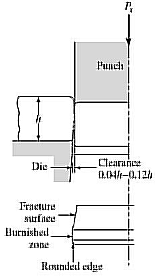
\includegraphics[width = 0.3\textwidth]{FrattLam1}}\quad
\subfloat[][\emph{Luce punzone-matrice troppo stretta}\label{fig:FrattLam2}]
{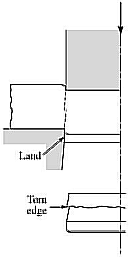
\includegraphics[width = 0.3\textwidth]{FrattLam2}}\quad
\subfloat[][\emph{Luce punzone-matrice troppo lasca}\label{fig:FrattLam3}]
{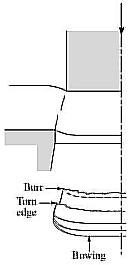
\includegraphics[width = 0.3\textwidth]{FrattLam3}}\\
\subfloat[][\emph{Schematizzazione della propagazione delle cricche in funzione della luce}
\label{fig:FrattLam4}]
{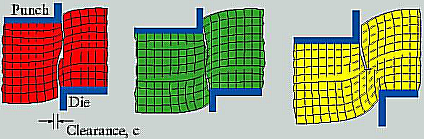
\includegraphics[width = 0.5\textwidth]{FrattLam4}}
\caption{Processo di generazione di fratture controllate su lamiera durante taglio}
\label{fig:FrattLam}
\end{figure}

Le fasi del taglio possono essere riassunte in tre fasi distinte:
\begin{description}
\item[I Fase]Quando i bordi degli utensili penetrano nella lamiera, questa viene prima spinta nella matrice e la deformazione plastica provoca un arrotondamento del suo bordo. 
La prima fase del taglio perciò è una piegatura dei bordi della lamiera, visibili nei disegni \ref{fig:FrattLam}, \eng{rounded edge} visibile in particolare nel disegno \ref{fig:FrattLam1}.
\item[II Fase] Quindi viene spinta nella matrice mediante deformazione plastica simile a un'estrusione, indicata da una zona brunita con striature parallele sulla superficie di taglio e caratterizzata da una forza in costante aumento, \eng{burnished zone} indicata al disegno \ref{fig:FrattLam1}. 
\item[III Fase] Dopo una certa deformazione critica, si generano fratture ad un leggero angolo rispetto alla direzione di taglio, di solito cominciando dal bordo della matrice.
Quando queste fratture si incontrano, la tranciatura è completa (\eng{fracture surface} sempre indicata al disegno \ref{fig:FrattLam1}). La forza di taglio scende anche se i bordi di taglio degli utensili sono entrati solo in parte nello spessore della lamiera. La nascita e propagazione delle cricche è la terza fase, che completa il taglio.
\end{description}

La superficie di frattura non è perpendicolare alla superficie del foglio e presenta una certa rugosità. Tuttavia, la finitura è accettabile per mole applicazioni.

La parte tagliata resterebbe attaccata alla matrice e deve essere spinta dal punzone oltre la parete verticale.
La qualità della superficie di taglio è fortemente influenzata dalla distanza tra i due bordi di taglio, chiamata \textbf{luce}. Con una luce molto piccola, le fratture che hanno origine dai bordi degli utensili non si incontrano e il taglio viene poi completato da un processo secondario di frattura, producendo un bordo frastagliato a circa metà dello spessore della lamiera (\eng{torn edge} nella figura \ref{fig:FrattLam2}).
Una luce eccessiva consente una deformazione plastica estesa, la separazione è ritardata e si forma un bordo superiore di bava tagliente (\eng{burr} al disegno \ref{fig:FrattLam3}).
Le figure a colori, \ref{fig:FrattLam4}, mostrano che la curvatura del bordo della lamiera aumenta con la luce.

Nel corso della tranciatura di migliaia di parti, i bordi degli utensili si usurano, si arrotondano e si forma un bordo frastagliato e tagliente anche con una luce ottimale.
Il bordo frastagliato della bava concentra gli sforzi; l'effetto nocivo è evidente nell'allungamento ridotto misurato nella prova di trazione.
La bava provoca l'innesco della frattura durante la deformazione successiva o in servizio, quindi una corretta scelta della luce e una manutenzione regolare degli utensili sono aspetti vitali del processo.
Una piccola luce conduce ad una usura più rapida degli utensili, pertanto la massima economia si ottiene quando la luce viene scelta più grande possibile compatibilmente con l'applicazione prevista. Ricordo che all'aumentare della luce aumenta anche la curvatura della lamiera.
In genere la luce è compresa tra il 4 e il 12\% dello spessore della lamiera (i valori inferiori si usano con i materiali più duttili).

\subsection{Valutazione delle forze sul taglio}
Si può facilmente valutare la forza della pressa necessaria per la tranciatura convenzionale. Poiché la deformazione è concentrata in una zona molto stretta con forte incrudimento, la forza massima può essere ottenuta da una tensione di taglio determinata sperimentalmente moltiplicata per la sezione trasversale da tagliare.
La tensione di taglio diminuisce all'aumentare della luce, ma i valori medi possono essere trovati nei manuali o possono essere considerati come una frazione $C_1$ del $UTS$, tensione massima a rottura, cioè la massima tensione nella curva tensione-deformazione nominale.
Così, la forza di taglio $P_s$ è data dalla formula:
\begin{equation}
P_s = C_1(TS) h l = C_1 K \left(\frac{n}{e}\right)^n hl
\label{eqn:ForzaTaglio}
\end{equation}
dove:\\
\begin{tabular}{cl}
$h$ & è lo spessore della lamiera\\
$l$ & è la lunghezza del taglio\\
$C_1$ & è $0.85$ per i materiali duttili e quelli $0.65$ i meno duttili\\
\end{tabular}\\
L'$UTS$ della maggior parte dei materiali è noto.
Se sono disponibili solo i valori K e n, l'$UTS$ può essere approssimato sostituendo 
\begin{equation}
UTS = K \left(\frac{n}{e} \right)^n
\end{equation}
dove $e$ è la base dei logaritmi naturali. 
Ricordando che la deformazione vale $n$ quando comincia a manifestarsi la strizione.
Quando i bordi di taglio sono paralleli, $l$ è l'intera lunghezza del profilo di taglio.

Ciò può portare a forze molto elevate, che possono quindi essere ridotte inclinando tra loro i due bordi di taglio, come in una ghigliottina, pertanto si deve considerare solo la lunghezza istantanea di taglio, come al disegno \ref{fig:ValForzeTaglio1}.
Nella tranciatura, il materiale di scarto può essere piegato e l'inclinazione è sullo stampo, come in figura \ref{fig:ValForzeTaglio2}. Nella punzonatura, per lo stesso motivo l'inclinazione è sul punzone, in figura \ref{fig:ValForzeTaglio3}. L'inclinazione è sempre simmetrica, in modo che la forza risultante sia verticale. In caso contrario la forza tenderebbe a spostare lateralmente la lamiera.
Alcune Possibili soluzioni sono quelle rappresentate alla figura \ref{fig:PunzoneInc}.

\begin{figure}
\centering
\subfloat[][\emph{Valutazione della pressione necessaria per eseguire un taglio}\label{fig:ValForzeTaglio1}]
{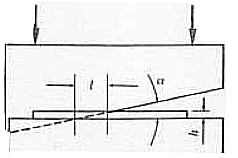
\includegraphics[width = 0.3\textwidth]{ValForzeTaglio1}}\quad
\subfloat[][\emph{Inclinazione matrice per diminuire la forza necessaria (tranciatura)}\label{fig:ValForzeTaglio2}]
{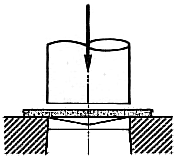
\includegraphics[width = 0.3\textwidth]{ValForzeTaglio2}}\quad
\subfloat[][\emph{Inclinazione del punzone per limitare le forze sull'utensile (punzonatura)}\label{fig:ValForzeTaglio3}]
{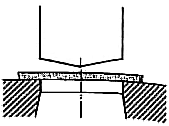
\includegraphics[width = 0.3\textwidth]{ValForzeTaglio3}}
\caption{Valutazione delle forze applicate per un taglio di lamiera e miglioramento delle forze applicate agli utensili}
\label{fig:ValForzeTaglio}
\end{figure}

In termini energetici: l'energia di tranciatura $E_s$ che la pressa deve fornire è uguale all'area sotto la curva forza-spostamento. Un valore approssimativo può essere ottenuto dalla formula:
\begin{equation}
E_s = C_2 P_s h
\end{equation}
dove $C_2 = 0.5$ per i materiali teneri e $0.35$ per i materiali duri.
Mentre $P_s$ è quella dell'equazione \eqref{eqn:ForzaTaglio}.

\begin{figure}
\centering
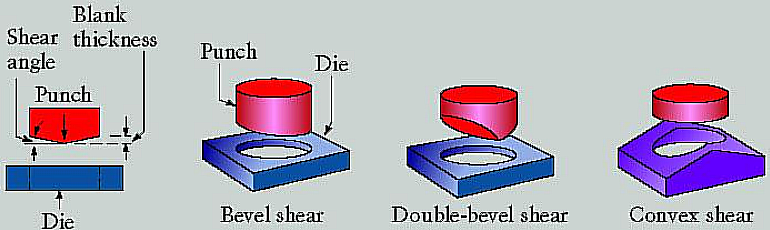
\includegraphics[width = \textwidth]{PunzoneInc}
\caption{Tipologie di sistemi punzone-matrice inclinati}
\label{fig:PunzoneInc}
\end{figure}

\subsection{Aspetti migliorativi}
Esiste una grande richiesta per processi che producano bordi tagliati di qualità, perpendicolari alla superficie della lamiera e con una finitura superficiale sufficientemente liscia per consentire l'uso immediato delle parti, ad esempio come ingranaggi in macchine con carichi limitati e tolleranze strette.
Sono possibili diversi approcci; nella maggior parte di essi, un contro-punzone collabora con il punzone principale e, come vantaggio aggiuntivo, elimina la curvatura della lamiera.

\begin{enumerate}
\item Abbiamo visto che la frattura può essere ritardata dall'imposizione di un'alta pressione idrostatica.
Questo principio viene sfruttato nella tranciatura fine. Un premi-lamiera appositamente sagomato viene premuto sulla lamiera appena prima di iniziare il taglio, così la zona in cui avviene la deformazione viene mantenuta in compressione e l'intero spessore viene tagliato senza che partano le cricche.
Tale tecnica è mostrata al disegno \ref{fig:PremiLamiera}.
\item Una pressione idrostatica elevata viene provocata anche tagliando con una luce negativa (interferenza) e la parte in effetti viene spinta (estrusa) attraverso la matrice, illustrato dal disegno \ref{fig:LuceNegativa}.
\item In qualche caso la lamiera viene bloccata tra due matrici. I punzoni penetrano in una direzione fino a quando non si generano le cricche, quindi il taglio viene completato nell'altra direzione. Illustrato al disegno \ref{fig:PunzControPunz}.
\item Una lamiera tranciata in modo convenzionale può subire una \textbf{rasatura} di finitura in un set di stampi con luce molto ridotta. In figura \ref{fig:TrancFine}.
\item La qualità del taglio migliora notevolmente nel taglio ad alta velocità quando le velocità di taglio superano la velocità di propagazione delle dislocazioni nel metallo. Ciò richiede velocità molto elevate, nell'ordine di $30 \unit{\m/\s}$.
\end{enumerate}

\begin{figure}
\centering
\subfloat[][\emph{Tranciatura fine tramite premi-lamiera}\label{fig:PremiLamiera}]
{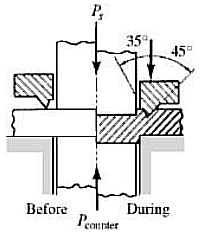
\includegraphics[width = 0.25\textwidth]{PremiLamiera}}
\subfloat[][\emph{Tranciatura fine tramite punzone a luce negativa}\label{fig:LuceNegativa}]
{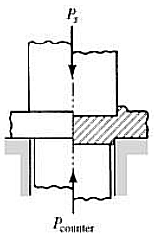
\includegraphics[width = 0.25\textwidth]{LuceNegativa}}
\subfloat[][\emph{Tranciatura fine tramite punzone e contro-punzone}\label{fig:PunzControPunz}]
{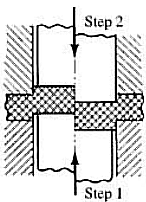
\includegraphics[width = 0.25\textwidth]{PunzControPunz}}
\subfloat[][\emph{Tranciatura fine tramite rasatura}\label{fig:TrancFine}]
{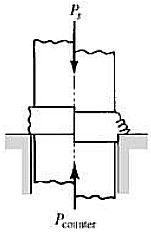
\includegraphics[width = 0.25\textwidth]{TrancFine}}
\caption{Esempi di tranciature fini in diversi metodi}
\label{fig:TranciaturaFine}
\end{figure}

Il punzone e la matrice sono fatti con acciaio per utensili o, per i lotti più grandi, con WC sinterizzato.
Il materiale di scarto (o, in punzonatura, la parte) si incastrerebbe sul punzone (o si infila nella matrice) e deve essere staccato con piastre di estrazione fisse, a molla o mosse da camme o con un cuscino di schiuma plastica (solitamente poliuretanica).
La scelta del processo è determinata principalmente dalle caratteristiche del prodotto e dalla dimensione del lotto di produzione.

\begin{figure}
\centering
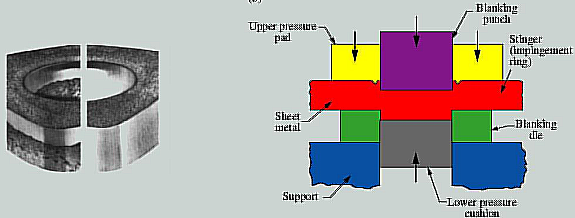
\includegraphics[width = \textwidth]{TranciaturaFine}
\caption{Confronto tra tranciatura semplice e tranciatura fine}
\label{fig:TanciaturaFine}
\end{figure}

Fori di dimensioni e forme standard possono essere tagliati su presse punzonatrici standard con utensili intercambiabili.

\subsection{Macchinari e tecniche di lavorazione}

La sostituzione della matrice viene accelerata con apparati rotanti nelle macchine a torretta.
Le punzonatrici \ac{CNC}, dotate di tavole x-y e di magazzini utensili, consentono un rapido e preciso posizionamento della lamiera e la selezione del punzone e della matrice, consentendo quindi la produzione a basso costo e flessibile di quantità piccole e medie.
I fori più grandi possono essere fatti con il taglio ripetuto con lo stesso punzone (roditura).
Geometrie complesse possono essere create in stampi composti in cui diversi bordi di taglio lavorano contemporaneamente.

Con gli stampi progressivi vengono eseguite in sequenza diverse operazioni di punzonatura e tranciatura con elementi degli stampi fissati a piastre comuni, mentre la striscia avanza di incrementi esatti. Spesso, la tranciatura e la punzonatura sono tra le numerose fasi di lavorazione eseguite in stampi progressivi che producono parti complesse.
La produttività è elevata, limitata solo dalla velocità di alimentazione del materiale nella pressa e dalla frequenza dei colpi della pressa (alcune presse operano a diverse centinaia di colpi al minuto). Ne è un esempio la figura \ref{fig:MatrProg}.

Punzoni multipli vengono utilizzati quando devono essere prodotte molte parti o fori, come nella tranciatura di cerchi per la produzione di lattine o di punzonatura di fori per lamiere forate.
Le velocità di produzione più alte sono ottenute quando la matrice e il punzone sono ricavati sulle superfici di rulli.

\begin{figure}
\centering
\subfloat[][\emph{Esempio di matrice progressiva}\label{fig:MatrProg}]
{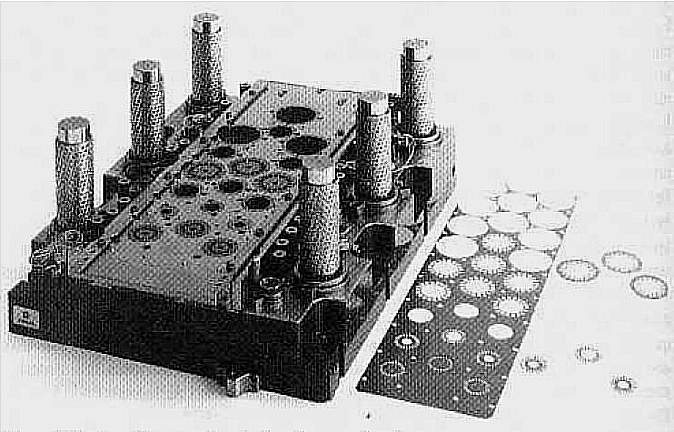
\includegraphics[width = 0.5\textwidth]{MatrProgr}}\\
\subfloat[][\emph{Esempio di tranciatura tramite cuscino in polieuretano}\label{fig:SteelPlatePunch}]
{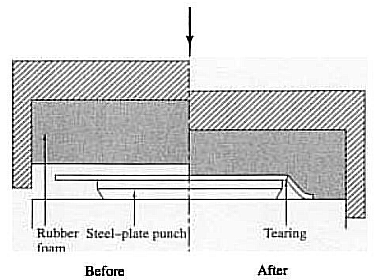
\includegraphics[width = 0.5\textwidth]{SteelPlatePunch}}
\caption{Processi di tranciatura per grandi e piccoli lotti}
\label{fig:ProcessoTranciatura}
\end{figure}

Per quantità minori o, ad esempio, poche centinaia di pezzi, il costo dello stampo può essere ridotto se è tollerabile una perdita di materiale maggiore.
Nella tranciatura con cuscino in gomma, la matrice è semplicemente una piastra in acciaio tagliata a misura (\eng{steel-plate punch} in figura \ref{fig:SteelPlatePunch}) e l'azione di taglio avviene premendo il foglio intorno a questo stampo con un cuscino in gomma. La parte sovrastante della lamiera è piegata e bloccata contro la piastra dal cuscino, e la rottura (\eng{tearing}) si verifica intorno ai bordi della piastra.

Per piccoli lotti, una soluzione economica è la fustella in acciaio. In questo caso, lo "stampo" è costituito da strisce di acciaio inossidabile o in acciaio ad alto tenore di carbonio con bordo inclinato dette fustella (\eng{steel rule} in figura \ref{fig:Fustella}), pressate in fessure in compensato (\eng{plywood}) mediante una piastra in acciaio (\eng{steel backing}).

Celle di punzonatura contengono una o due punzonatrici o centri di punzonatura e un qualche meccanismo di trasferimento. Il carico delle lamiere, il cambio utensile, il trasferimento di parti tra le macchine e lo scarico della parte sono coordinati mediante automazione flessibile.

Il processo di taglio può essere adattato per fili, barre, profili e tubi in preparazione per ulteriori processi. La qualità del taglio è migliorata fornendo supporto per il pezzo da tagliare e anche applicando tensione di compressione (pressione idrostatica) durante il taglio.

C'è stato un rapido sviluppo di metodi di taglio basati su tecniche di saldatura (raggio laser, fascio elettronico, torcia al plasma, arco elettrico o ossitaglio e taglio a getto d'acqua. Combinati con tavole x-y (e talvolta presse a torretta), tali centri di taglio controllati da computer diventano estremamente versatili e produttivi e non richiedono l'uso di stampi.

\begin{wrapfloat}{figure}{O}{0pt}
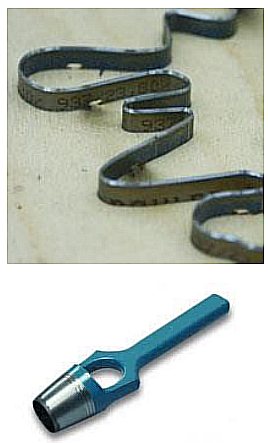
\includegraphics[width = 0.3\textwidth]{Fustella}
\caption{Esempi di \eng{Steel-rule} e fustella}
\label{fig:Fustella}
\end{wrapfloat}

\section{Piegatura delle lamiere}
Molte lamiere vengono piegate. Caratteristica di questo processo è l'allungamento imposto sulla superficie esterna e la compressione sulla superficie interna.
Per uno specifico spessore della lamiera $T$, le deformazioni di trazione e compressione aumentano al diminuire del raggio di formatura $R$, più precisamente al diminuire del rapporto $R/T$, dove $T$ è lo spessore.
Affinché il ritorno elastico sia trascurabile e la lamiera mantenga la forma anche tolto il carico, il rapporto $R/T$ deve essere sufficientemente piccolo da portare gran parte della sezione della lamiera a deformarsi plasticamente.
C'è, come nella piegatura elastica, solo una linea (\textbf{l'asse neutro}) che mantiene la sua lunghezza originale.

Quando si piega con raggi abbastanza grandi, l'asse neutro è al centro. Quando si piega con raggi piccoli, l'asse neutro si sposta verso la parte in compressione, la linea centrale si allunga e la costanza del volume viene preservata dall'assottigliamento della lamiera.
L'aumento della lunghezza della linea centrale viene di solito preso in considerazione per le pieghe in cui $R < 2T$ assumendo che l'asse neutro sia posizionato ad un terzo dello spessore della lamiera.
Quando la lamiera è relativamente stretta ($L/T < 8$, dove L è la larghezza di piega), c'è anche una contrazione in larghezza.

\begin{figure}
\centering
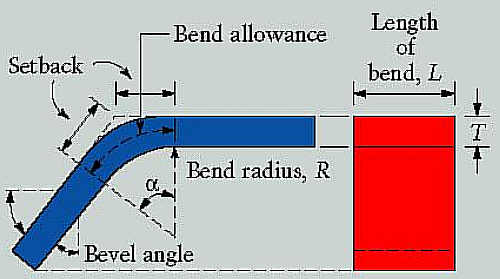
\includegraphics[width = \textwidth]{PiegaLam}
\caption{Parametrizzazione della piega sulle lamiere}
\label{fig:PiegaLam}
\end{figure}

Il raggio minimo di piega (il più piccolo raggio di matrice consentito $R$ o, più correttamente, il rapporto minimo tra raggio e spessore $R/T$) può essere definito secondo diversi criteri.
\pagebreak
\begin{enumerate}
\item La buccia d'arancia può essere esteticamente indesiderabile ma non è un difetto poiché può essere risolto scegliendo un materiale a grana fine.
\item La strizione localizzata provoca un indebolimento strutturale della lamiera piegata.
La strizione avviene quando l'allungamento della fibra esterna supera l'allungamento uniforme del materiale $e_u$ nella prova di trazione. Nella formula \eqref{eqn:StrizLocal} $R_b$ è il raggio di piega e $h$ lo spessore della lamiera
\item La frattura rappresenta un limite assoluto. Questa è direttamente correlata alla riduzione dell'area $q$ misurata alla rottura nella prova di trazione. Il raggio minimo di piega consentito può essere stimato per materiali meno duttili dalla \eqref{eqn:LowDuct} e per i materiali duttili, a causa dello spostamento del raggio neutro nelle pieghe strette,
dalla \eqref{eqn:HighDuct}.
Di solito un materiale con $q > 0.5$ può essere piegato su se stesso, si parla allora di raggio di piega zero.
\begin{align}
R_b &= k \left(\frac{1}{2q}\right)-1 & \text{con } q <0.2 \label{eqn:LowDuct}\\
R_b &= h\frac{(1-q)^2}{2q-q^2} & \text{con } q >0.2 \label{eqn:HighDuct}
\end{align}
\item Con raggi molto piccoli può verificarsi schiacciamento sulla superficie interna e formazione di pieghe.
\end{enumerate}

La strizione localizzata può essere descritta come:
\begin{equation}
e_t = \frac{1}{(2R_b / h) + 1} \leq e_u
\label{eqn:StrizLocal}
\end{equation}

Per i materiali il cui comportamento può essere approssimato con legge esponenziale \eqref{eqn:Def-Sforzo}, 
\begin{equation}
\sigma = K \epsilon^n
\label{eqn:Def-Sforzo}
\end{equation}
$\epsilon_u = n$ e la deformazione uniforme ingegneristica $e_u$ può essere ottenuta dalla formula \eqref{eqn:AllungamentoUniforme}.
\begin{equation}
e_u = \left(\exp(n)\right) - 1
\label{eqn:AllungamentoUniforme}
\end{equation}

La relazione è più affidabile con gli acciai; per la maggior parte degli altri materiali, dovrebbe essere utilizzato l'effettiva $e_u$ misurata nella prova di trazione.
Poiché la deformazione viene redistribuita alle zone adiacenti durante la piega, è generalmente permessa una deformazione un po' più elevata.
Un collare di bava provoca un aumento di tensione e, se sulla superficie esterna (a trazione), porta a frattura molto prima. Pertanto, se possibile, il collare è orientato verso il punzone, dove il materiale è sottoposto a compressione.

L'anisotropia, di qualsiasi tipo, influenza la piegatura. Un orientamento preferenziale delle fibre produce una maggiore duttilità nella direzione di laminazione, perciò conviene piegare le lamiere con la linea di piega ortogonale alla direzione di laminazione, come è mostrato nelle figure \ref{fig:BendCracked}.
Un materiale con basso valore di $r$ caratterizzato da tessitura si assottiglia facilmente e quindi può essere piegato con raggi più piccoli di un materiale con alto valore di $r$. Questa è una delle non numerose situazioni in cui convenga avere $r$ piccolo. Ricordando che $r$ è il rapporto tra deformazione nello spessore e rapporto in larghezza nella prova di trazione. La foto \ref{fig:RealCrack} mostra cricche sulla superficie di una lamiera piegata e il restringimento ai bordi.

\begin{figure}
\centering
\subfloat[][\emph{Esempio di piega parallela alla laminazione con conseguente fratture della superficie}\label{fig:CrackedBend}]
{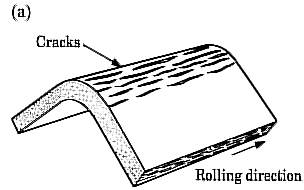
\includegraphics[width = 0.4\textwidth]{CrackedBend}}\quad
\subfloat[][\emph{Esempio di piega ortogonale alla direzione della laminazione}\label{fig:OKBend}]
{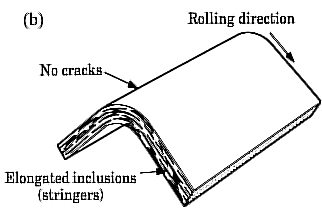
\includegraphics[width = 0.4\textwidth]{OKBend}}\\
\subfloat[][\emph{Foto reale di lamiera piegata con fratture}\label{fig:RealCrack}]
{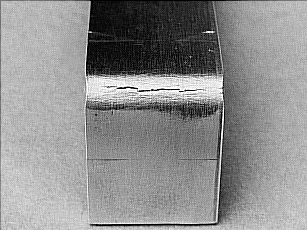
\includegraphics[width = 0.5\textwidth]{RealCrack}}
\caption{Generazione di fratture durante la piegatura}
\label{fig:BendCracked}
\end{figure}

\subsection{Stato delle tensioni residue}
Lo stato tensionale è estremamente complesso nella piegatura.
Partendo dall'asse neutro, il materiale è soggetto a una deformazione crescente fino alle 2 superfici, da una parte in trazione e dall'altra in compressione. Ciò significa che intorno all'asse neutro le deformazioni sono elastiche.
Quando si toglie la forza usata per piegare, il momento dovuto alla parte di materiale
deformato solo elasticamente causa il ritorno elastico, e provoca la formazione di una
distribuzione di tensioni residue. Il ritorno elastico delle lamiere è chiamato \eng{springback}.

In riferimento alla figura \ref{fig:StatoTensioniResidue} (a) mostra una distribuzione triangolare. In campo elastico tale distribuzione è rappresentativa sia dello stato tensionale che di quello deformativo perché c'è proporzionalità tra tensione e deformazione. Nella figura \ref{fig:StatoTensioniResidue} (b) la distribuzione ha una forma diversa. Siccome la deformazione aumenta linearmente allontanandosi dall'asse neutro, quella in figura è sicuramente la distribuzione delle tensioni ed è stato superato lo snervamento in parte dello spessore. Nella figura \ref{fig:StatoTensioniResidue} (c), allo stato tensionale mostrato in \ref{fig:StatoTensioniResidue} (b) è stato sovrapposto lo stato tensionale dovuto allo scarico della forza che come si sa, avviene lungo una semiretta nel piano tensione/deformazione, perciò provoca una distribuzione triangolare. La somma delle 2 è mostrata in \ref{fig:StatoTensioniResidue} (d) e rappresenta la distribuzione risultante di
tensioni residue.
Lo \eng{springback} stabilisce un nuovo equilibrio di forze con una distribuzione di tensioni residue
caratterizzata da tensioni di compressione all'esterno e di trazione sulla superficie interna.

\begin{figure}
\centering
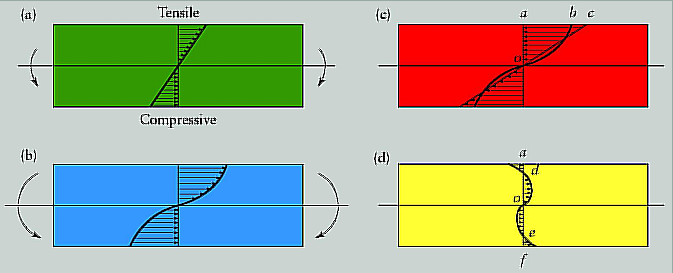
\includegraphics[width = \textwidth]{StatoTensioniResidue}
\caption{Stato delle tensioni residue}
\label{fig:StatoTensioniResidue}
\end{figure}

Lo \eng{springback} recupera elasticamente parte della deformazione totale; in particolare, aumenta il raggio e riduce l'angolo della parte piegata.
La zona elastica è più ampia per una piega relativamente dolce (grande rapporto $R_b/h$, dove $R_b$ è il raggio di piega e $h$ lo spessore) e per un materiale con un elevato rapporto tra tensione di snervamento $\sigma_{0.2}$ e modulo elastico $E$. Lo \eng{springback} può essere espresso mediante la formula \eqref{eqn:SpringBack};
\begin{align}
\frac{R_b}{R_f} &= 1 - 3 \left(\frac{R_b}{h}\frac{\sigma_{0.2}}{E}\right) + 4\left(\frac{R_b}{h}\frac{\sigma_{0.2}}{E}\right)^3
\label{eqn:SpringBack}\\
\alpha_f &\left(R_f+\frac{h}{2}\right) = \alpha_b \left(R_b + \frac{h}{2}\right)
\label{eqn:AngoloSprinback}
\end{align}
dove $R_b$ è il raggio della matrice di piegatura e $R_f$ è il raggio ottenuto dopo aver tolto la pressione di formatura.
Poiché la lunghezza dell'asse neutro non cambia, l'angolo dopo lo \eng{springback}, $\alpha_f$ può essere ottenuto in radianti dalla formula \eqref{eqn:AngoloSprinback} che esprime appunto l'invarianza della lunghezza dell'asse neutro da quando viene applicato il carico alla fase dopo lo scarico.
Al disegno \ref{fig:SpringBack} vengono rappresentati i parametri.

\begin{figure}
\centering
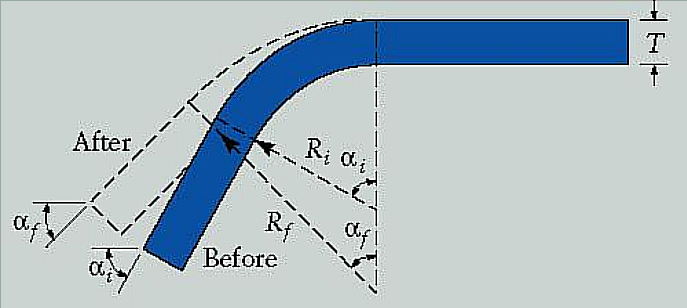
\includegraphics[width = \textwidth]{SpringBack}
\caption{Parametri per valutare lo \eng{springback}}
\label{fig:SpringBack}
\end{figure}

Diverse tecniche sono utilizzate per combattere lo \eng{springback}, rispettivamente in figura \ref{fig:SolSpringback}:
\begin{enumerate}
\item Se è noto lo \eng{springback} per un determinato materiale e se il materiale è di qualità e spessore uniforme, è possibile compensare piegando più del voluto. Questa è la forma di piegatura più semplice, in cui non viene applicata alcuna pressione di compressione nella direzione dello spessore della lamiera, si parla di \textbf{piegatura in aria}.
\item Negli altri casi la soluzione consiste nel fare in modo che tutto il materiale nella zona di piega venga deformato plasticamente. La zona elastica può essere eliminata alla fine della corsa del punzone con due tecniche.
	\begin{itemize}
	\item Innanzitutto, le due estremità della lamiera possono essere bloccate prima che il punzone scenda, in modo che la corsa del punzone provochi lo stiramento della lamiera, causando snervamento a trazione nell'intero spessore della lamiera. Nessuna figura riproduce questa soluzione.
	\item Nel secondo metodo il naso del punzone è sagomato per indentare la lamiera, in modo che la compressione plastica avvenga in tutto lo spessore.
	\end{itemize}
\item Se si utilizza un contro-punzone con una pressione controllata, le tensioni di compressione vengono mantenute nella zona della piega durante l'intero processo. Poiché questo ha anche l'effetto di imporre una pressione idrostatica sulla zona di curvatura, è possibile flettere il materiale oltre i suoi limiti naturali.
\item I materiali meno duttili possono essere piegati ad una temperatura elevata; poiché la tensione di snervamento è più bassa, anche lo \eng{springback} è minore.
\end{enumerate}

\begin{figure}
\centering
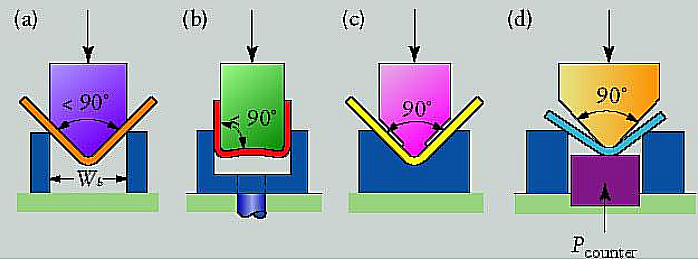
\includegraphics[width = \textwidth]{SolSpringback}
\caption{Soluzioni migliorative allo \eng{springback}}
\label{fig:SolSpringback}
\end{figure}

\subsection{Valutazione della forza di piegatura}
Una semplice stima della forza di piegatura in piegatura libera a 90 ° può essere ottenuta dalla formula:
\begin{equation}
P_b = \frac{wh^2 (TS)}{W_b}
\end{equation}
Dove $W_b$ è la larghezza dell'apertura della matrice e $w$ la larghezza della striscia (la lunghezza della linea su cui si effettua la piegatura).

\subsection{Macchinari e tecniche di lavorazione}
\begin{wrapfloat}{figure}{O}{0pt}
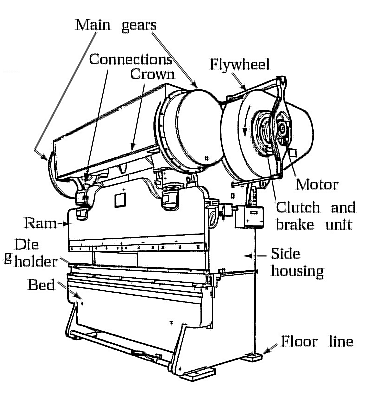
\includegraphics[width = 0.4\textwidth]{PressaPiegatrice}
\caption{Esempio di pressa piegatrice}
\label{fig:PressaPiegatrice}
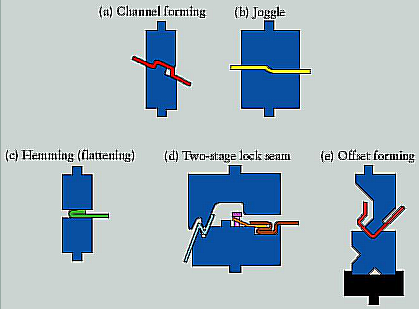
\includegraphics[width = 0.4\textwidth]{UtensiliPiegatura}
\caption{Varietà di utensili utilizzabili per la piegatura delle lamiere}
\label{fig:UtensiliPiegatura}
\end{wrapfloat}

La macchina utilizzabile per la piegatura dipende dalla dimensione, per lo più dalla larghezza della lamiera piegata.
Le p[resse meccaniche, viste parlando di forgiatura ed estrusione, possono piegare lamiere strette ad alta velocità.
le presse piegatrici sono presse speciali con supporti molto lunghi. IN queste, semplice utensili vengono utilizzati per realizzare forme complesse piegando ripetutamente una lamiera lunga.
I costi possono essere ridotti quando una lastra in schiuma di poliuretano sostituisce lo stampo femmina.
Un esempio di pressa piegatrice è quella della figura \ref{fig:PressaPiegatrice}.

Una grande varietà di forme può essere prodotta con un numero limitato di utensili, come si può vedere dalla figura \ref{fig:UtensiliPiegatura}. 
La deflessione elastica dell'attrezzatura (che si apre al centro sotto la forza della pressa) provocherebbe variazioni dell'angolo di piega, pertanto gli stampi devono essere realizzati in modo che pieghino di più al centro.
Questo si ottiene spessorando o, nelle presse moderne, mediante flessione meccanica o idraulica, spesso sulla base di forze di piega calcolate.

\begin{figure}
\centering
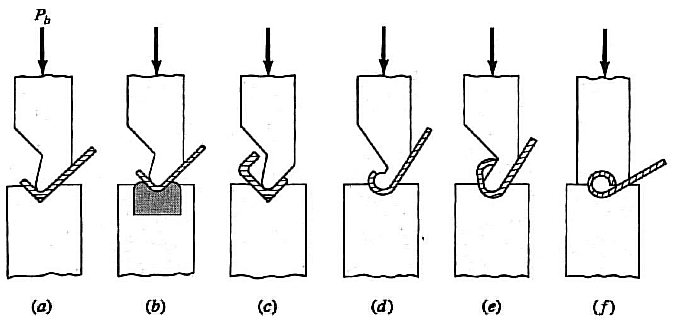
\includegraphics[width = \textwidth]{ProcessoPiegatura}
\caption{Alcune sezioni di utensili per la piegatura}
\label{fig:PreocessoPiegatura}
\end{figure}

Le figure \ref{fig:ProcessoTranciatura} mostrano altre operazioni eseguibili su pressa piegatrice. Le figure da d ad f illustrano una sequenza di piegatura.
In combinazione con alimentatori di lamiera meccanizzati, la pressa è adatta ad essere controllata da computer, compreso un riscontro per rilevare la posizione della lamiera. La compensazione per lo \eng{springback} è fatta con l'aiuto di tabelle o equazioni empiriche.
Schemi di controllo più sofisticati prendono in considerazione le proprietà del materiale. In un caso, l'angolo di piega viene misurato nella prima corsa; la forza viene quindi rilasciata per ottenere lo \eng{springback} e viene effettuata una seconda corsa di compensazione.
In altri schemi, la curva elasto-plastica tensione-deformazione è derivata da informazioni ottenute con trasduttori di forza e di spostamento e un algoritmo di controllo calcola l'incremento di piega richiesta.

La piegatura con pressa pannellatrice, mostrata in figura \ref{fig:PressaPannellatrice}, è un metodo alternativo per piegare. Per stimare la forza di piegatura, $W_b$ può essere considerata come $(2R + h)$. La pressa pannellatrice può piegare solo in prossimità dei bordi della lamiera e, a parità di altri fattori, deve applicare una forza maggiore rispetto alla pressa piegatrice. In compenso il posizionamento della lamiera è più preciso e il tempo ciclo è inferiore.

La piegatura con tre rulli impartisce una curvatura uniforme ma regolabile a lamiere, piastre o profili deformando con rulli disposti in modo piramidale. Si tratta di un'importante fase di preparazione per realizzare grandi anelli e strutture saldate. La macchina si chiama \textbf{calandra} e \textbf{calandratura} l’operazione.
Illustrata in figura \ref{fig:PiegaRulli}

\begin{figure}
\centering
\subfloat[][\emph{Esempio di pressa pannellatrice}\label{fig:PressaPannellatrice}]
{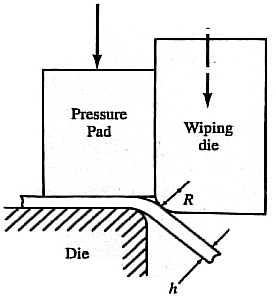
\includegraphics[width = 0.4\textwidth]{PressaPannellatrice}}\quad
\subfloat[][\emph{Schema di realizzazione della piegatura tramite rulli}
\label{fig:PiegaRulli}]
{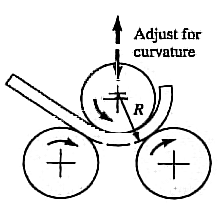
\includegraphics[width = 0.4\textwidth]{PiegaRulli}}
\caption{Ulteriori tecniche di piegatura}
\label{fig:TecPiega}
\end{figure}

La formatura a rulli è un metodo di produzione molto veloce. La piegatura è ora fatta progressivamente, passando la striscia tra rulli sagomati, a coppie. Prodotto tipici sono le lamiere ondulate e i guard-rail.
Per molte altre forme, rulli folli sono usati per premere i lati della forma parzialmente deformata.
In questo modo possono essere formati anche tubi da saldare successivamente, profili che sostituiscono sezioni laminate a caldo o estruse, nonché forme complesse (come i telai per porte).

La curvatura di profili e tubi è un'importante attività produttiva. Il problema della piegatura libera è legato al fatto che le forme più complesse possono distorcersi e accartocciarsi. Risultati migliori sono ottenuti quando la sezione o il tubo sono avvolti attorno ad una forma rigida, come mostrato nelle figure.

\begin{figure}
\centering
\subfloat[][\emph{Pressaggio di profili complicati}\label{fig:ProfComplex}]
{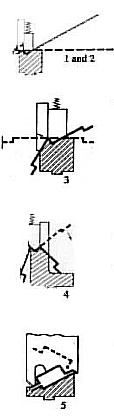
\includegraphics[width = 0.2\textwidth]{PiegaAuto1}}\quad
\subfloat[][\emph{Realizzazione di profili per strisciamento}
\label{fig:ProfStrisciamento}]
{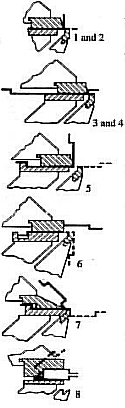
\includegraphics[width = 0.2\textwidth]{PiegaAuto2}}\quad
\subfloat[][\emph{Ottenimento di profili tramite rulli}
\label{fig:ProfRulli}]
{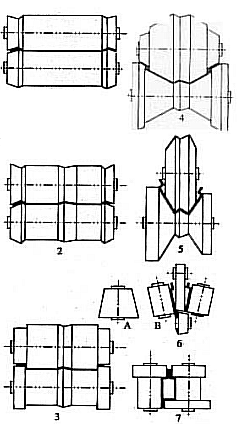
\includegraphics[width = 0.4\textwidth]{PiegaAuto3}}
\caption{Ottenimento di profili di forme decisamente variegata, su macchine automatiche}
\label{fig:PiegaAuto}
\end{figure}

L'adeguamento alla forma è garantito dall'avvolgimento sotto trazione, passando attorno al profilo o al tubo un rullo strisciante \ref{fig:PiegaTubi}, un blocco fissato al centro curvatura o da una forma rigida rotante \ref{fig:PiegaTubiFine}.
Per evitare il collasso dei tubi nella curvatura su raggi stretti, sono disponibili diversi metodi.
L'interno è supportato con sabbia, con un metallo a basso punto di fusione o, più economicamente, da un mandrino costituito da singole sezioni o il tubo è tirato su un mandrino fisso \ref{fig:PiegaSoffietti}.
Le piegatrici \ac{CNC} possono essere programmate per realizzare tubi con diverse curve in differenti orientamenti, come richiesto per sistemi idraulici di auto e aerei e scarichi automobilistici.

\begin{figure}
\centering
\subfloat[][\emph{Piegatura di tubi con deformazione della sezione}\label{fig:PiegaTubi}]
{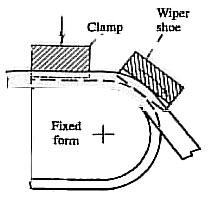
\includegraphics[width = 0.3\textwidth]{PiegaTubi}}\quad
\subfloat[][\emph{Piega dei tubi con supporto interno per evitare il collasso delle pareti}
\label{fig:PiegaTubiFine}]
{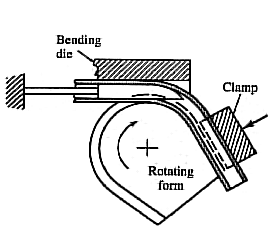
\includegraphics[width = 0.3\textwidth]{PiegaTubiFine}}\quad
\subfloat[][\emph{Inserto per realizzare dei tubi a soffietto}
\label{fig:PiegaSoffietti}]
{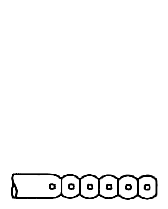
\includegraphics[width = 0.3\textwidth]{PiegaSoffietti}}
\caption{Tecniche di piegatura dei tubi}
\label{fig:TecPiegaTubi}
\end{figure}

\section{Stretch Forming}
Grandi quantità di lamiera sono deformate per realizzare componenti a forma di contenitori più o meno profondi, con una grande varietà di forme. In contrasto con la maggior parte dei componenti in lamiera piegati, sono caratterizzate da curvature in due direzioni (sono forme 3-D). Possono essere prodotte con lo \eng{stretch forming}, con un'imbutitura o con loro combinazioni. Nello \eng{stretch forming} puro la lamiera è completamente bloccata sul suo perimetro e la forma è sviluppata interamente a scapito dello spessore della lamiera. Fisicamente questo può essere ottenuto in diversi modi:

\begin{enumerate}
\item La lamiera può essere bloccata con un gran numero di morsetti fissi o rotanti.
Il vantaggio è che solo uno stampo (stampo maschio o punzone di forma) è necessario, ma la produttività è bassa; di conseguenza, tale operazione è più adatta per la produzione di bassi volumi come è tipico dell'industria aeronautica. Un'operazione di questo tipo è mostrata in figura \ref{fig:StretchForming1}.
Possono essere formate parti molto grandi (pelli di fusoliera, pelli d'ala, scafi per barche).
Il ritorno elastico può essere sostanziale realizzando forme con curvatura dolce; per risolvere il problema si può lavorare a temperature elevate (a volte sfruttando il \eng{creep} o la formatura superplastica del materiale).
Anche i profili laminati ed estrusi possono essere lavorati in questo modo.
\item Per la produzione di massa, per esempio nell'industria automobilistica e degli elettrodomestici, il semilavorato è bloccato con un premi-lamiera mobile indipendente che blocca il foglio con l'ausilio di rompi-grinze; il punzone assieme alla matrice femmina definiscono la forma. Questa tecnica è mostrata in figura \ref{fig:StretchForming2}.
Un prodotto è realizzato ad ogni corsa della pressa; quindi la produttività è alta ma anche i costi di produzione sono più alti.
\item Nel processo di stampaggio in rilievo il vincolo è dato dalla lamiera stessa, attraverso i punti di contatto multipli con la matrice. In questo caso di solito la deformazione è localizzata. Un esempio è mostrato in figura \ref{fig:StretchForming3}.
\end{enumerate}

\begin{figure}
\centering
\subfloat[][\emph{\eng{Stretch forming} tramite tiranti multipli}\label{fig:StretchForming1}]
{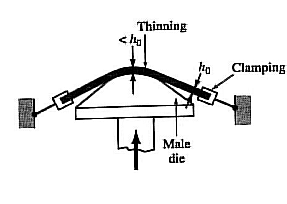
\includegraphics[width = 0.3\textwidth]{StretchForming1}}\quad
\subfloat[][\emph{\eng{Stretch forming} per produzioni massive}\label{fig:StretchForming2}]
{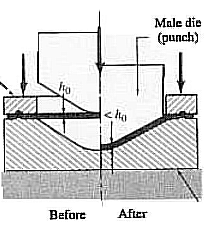
\includegraphics[width = 0.3\textwidth]{StretchForming2}}\quad
\subfloat[][\emph{\eng{Stretch forming} a deformazione localizzata}\label{fig:StretchForming3}]
{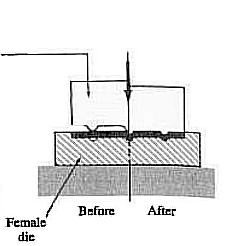
\includegraphics[width = 0.3\textwidth]{StretchForming3}}
\caption{Possibilità di \eng{Stretch forming} per l'industria}
\label{fig:StretchForming}
\end{figure}

\subsection{Deformabilità nello stretch forming}
Il primo limite viene raggiunto quando una strizione localizzata diventa visibile, invece il limite ultimo è dato dalla successiva frattura.
Il limite di formabilità è una proprietà tecnologica, perciò si usano prove di questo tipo per determinarla, in contrapposizione alle prove meccaniche che sono stabilite da normativa. La deformazione limite dipende dal materiale, dalla velocità di deformazione e dall'attrito sulla superficie del punzone.
I fattori che influenzano la deformazione limite diventano evidenti quando una lamiera bloccata sul perimetro viene allungata da un punzone semisferico, come è mostrato nella figura \ref{fig:TestTecStretch}.

Le variazioni di deformazione localizzate (la distribuzione della deformazione) possono essere rivelate semplicemente applicando una griglia di piccoli cerchi (generalmente di 2-6 mm di diametro) o una griglia di quadrati e cerchi sulla superficie della lamiera, di solito mediante incisione elettrolitica (tecnica di marcatura per materiali conduttori) o una tecnica a base di \eng{fotoresist} (materiale sensibile alla luce), come quelle che si usano in elettronica per la produzione di circuiti stampati. Si ottiene una superficie come quella mostrata in figura \ref{fig:MisuraTestStretch}.
Durante la deformazione, l'assottigliamento del materiale è accompagnato da una crescita dei cerchi, come richiesto dalla costanza del volume.
Quando la deformazione è la stessa in tutte le direzioni, come soffiando in un palloncino (deformazione biassiale simmetrica), il cerchio si espande in un cerchio di diametro maggiore.
Quando la deformazione è diversa in direzioni diverse, il cerchio si distorce in un'ellisse: l'asse maggiore dà la deformazione maggiore e, perpendicolare ad esso, l'asse secondario dà la deformazione minore.

\begin{wrapfloat}{figure}{O}{0pt}
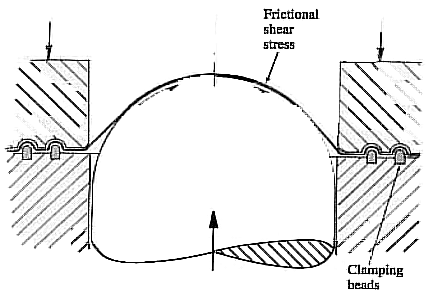
\includegraphics[width = 0.4\textwidth]{TestTecStretch}
\caption{Esempio di test tecnologico per lo \eng{stretch forming}}
\label{fig:TestTecStretch}
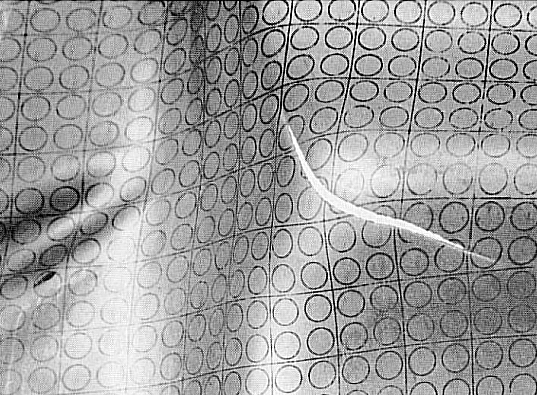
\includegraphics[width = 0.4\textwidth]{MisuraTestStretch}
\caption{Griglia di rilevazione di deformazioni localizzate}
\label{fig:MisuraTestStretch}
\end{wrapfloat}

Quando una lamiera di un determinato materiale viene allungato sul punzone semisferico, la distribuzione della deformazione dipende da un certo numero di fattori:
\begin{enumerate}
\item Nella totale assenza di attrito (che in realtà può essere realizzata solo nell'espansione idraulica), la lamiera si assottiglia gradualmente soprattutto sull'apice, dove infine si verifica la frattura.
Con un materiale avente un alto valore di n, si può ottenere una cupola più alta prima che la strizione diventi localizzata. Ricordando che nella prova di trazione la strizione avviene a $\epsilon = n$. Nella trazione biassiale simmetrica, la presenza di 2 deformazioni uguali tra loro ortogonali nel piano della lamiera, impedisce la formazione di una strizione localizzata, si ha perciò strizione diffusa.
\item L'attrito sulla superficie del punzone impedisce il libero assottigliamento sulla sommità e con un attrito crescente la posizione della massima deformazione si allontana dalla sommità. La deformazione diventa più localizzata e la frattura si verifica in condizioni di deformazione piana, dove lamiera e punzone vengono in contatto o in prossimità di tale punto.
\item In condizioni identiche, una lamiera più spessa si allunga maggiormente, perché la piegatura sovrapposta all'allungamento aumenta la duttilità.
\item L'entità dell'allungamento aumenta con tutte le variabili del materiale che ritardano la strizione (valore alto di n, trasformazioni) o aumentano la deformazione dopo strizione (valore alto di m). Infatti, si riscontra una buona correlazione empirica tra allungamento totale nella prova di trazione e altezza massima della cupola.
La distribuzione della deformazione è importante perché determina le proprietà della lamiera allungata
\end{enumerate}

La deformazione può continuare fino a quando si sviluppa una strizione localizzata in corrispondenza o in prossimità della sommità, in un punto in cui ci sia qualche disomogeneità nel materiale o la lamiera sia originariamente più sottile. Durante l'allungamento su un punzone, l'entità dell'allungamento non raggiunge mai quella ottenuta nell'espansione idraulica senza attrito, ma fintantoché l'attrito è molto basso, la rottura si verifica ancora sulla sommità.

\section{Imbutitura}
Anche l'imbutitura come lo stretching viene usata per produrre contenitori a partire da una lamiera piana. La differenza tra stretching e imbutitura è sostanziale: nel primo, il semilavorato è bloccato e la profondità è raggiunta a scapito dello spessore della lamiera; in quest'ultimo, al semilavorato è permesso - e persino è incoraggiato - ad entrare nella matrice, e lo spessore è nominalmente invariato.
Nel caso più semplice di imbutitura pura, un semilavorato circolare del diametro $d_0$ viene convertito in una contenitore a fondo piatto, trascinandolo su una matrice con l'aiuto di un punzone di diametro $D_p$.
Sia la matrice che il punzone devono avere bordi ben arrotondati, altrimenti il semilavorato potrebbe essere tagliato.

\begin{wrapfloat}{figure}{O}{0pt}
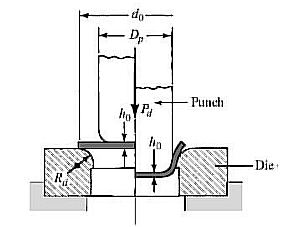
\includegraphics[width = 0.4\textwidth]{Imbutitura}
\caption{Schema di realizzazione dell'imbutitura}
\label{fig:Imbutitura}
\end{wrapfloat}\

Il contenitore finito viene estratto dal punzone, ad esempio, lavorando un leggero recesso nella parte inferiore della matrice.
Dopo che il contenitore è stato spinto attraverso la matrice, il suo bordo superiore si allarga a causa dello \eng{springback}, viene bloccato dalla sporgenza durante la corsa di ritorno del punzone e la sporgenza stacca il contenitore. Nel punzone spesso è presente un foro centrale per impedire la formazione di una depressione e pertanto aiuta il distacco.

\subsection{Imbutitura senza premi-lamiera}
Quando la porzione di lamiera sulla matrice scorre verso il foro nella matrice può dare luogo a pieghe chiamate grinze. La formazione di pieghe può essere evitata quando la lamiera è sufficientemente rigida. Questo si verifica sempre con imbutiture poco profonde, quando il rapporto di imbutitura \eqref{eqn:RappImbutitura}, dove $d_0$ è il diametro iniziale della lamiera e $D_p$ il diametro del punzone.
\begin{equation}
d_0/D_p <1.2 \label{eqn:RappImbutitura}
\end{equation}

Lamiere con spessore elevato rispetto al diametro iniziale consentono un rapporto di imbutitura maggiore; la formazione di pieghe dipende anche dal profilo della matrice, che determina la compressione circonferenziale. Il profilo più favorevole è la matrice a trattrice.
Il grafico \ref{fig:LimitiImbutitura} confronta le prestazioni di 3 diversi profili della matrice di imbutitura, troncoconico, cilindrico raccordato e a trattrice, mostrati a destra. La parte inferiore del grafico, identificata come \eng{good} rappresenta le imbutiture eseguibili senza formazione di grinze, la parte superiore (\eng{wrinkling}) dice quali imbutiture darebbero luogo alla formazione di grinze.

\begin{figure}
\centering
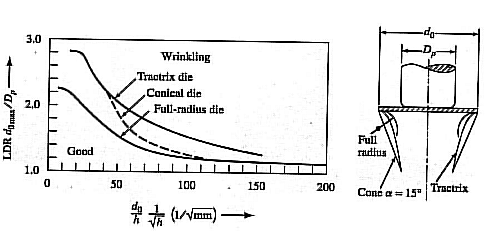
\includegraphics[width = \textwidth]{LimitiImbutitura}
\caption{Grafico coi limiti di imbutitura in funzione di un parametro geometrico}
\label{fig:LimitiImbutitura}
\includegraphics[width = \textwidth]{ProcImbutitura}
\caption{Sequenza degli eventi durante la corsa del punzone}
\label{fig:ProcImbutitura}
\end{figure}

Le figure \ref{fig:ProcImbutitura} mostrano la progressione di un'imbutitura in una matrice trattrice.
L'equazione \eqref{eqn:LimImbutitura} indica una condizione che deve essere rispettata per non produrre grinze.

\begin{equation}
D_0 - D_p < 5T
\label{eqn:LimImbutitura}
\end{equation}

\subsection{Imbutitura con premi-lamiera}
Quando la lamiera è relativamente sottile e il rapporto di imbutitura è oltre i limiti indicati
precedentemente, la flangia deve essere vincolata con un premi-lamiera, come si vede nella 
figura a sinistra. Il premi-lamiera deve esercitare pressione sufficiente per prevenire le pieghe, ma una pressione eccessiva limiterebbe il libero movimento del materiale e 
causerebbe fratture nella parete del contenitore. 
Per produrre un contenitore senza difetti, la pressione del premi-lamiera può essere presa, 
come prima approssimazione, pari al $1.5\%$ della tensione di snervamento del materiale.
Le foto \ref{fig:Imbutiti} mostrano la lamiera prima dell'imbutitura e 3 imbutiti. Nel caso (b) la pressione del premi-lamiera è insufficiente, in (c) è ottimale, in (d) è eccessiva. Nella figura (c) si vede anche la formazione delle orecchie, dovute all'anisotropia planare del materiale.

\begin{figure}
\centering
\includegraphics[width = \textwidth]{Imbutiti}
\caption{Casi di imbutiti con diverse pressioni del premi-lamiera}
\label{fig:Imbutiti}
\end{figure}

\subsection{Valutazione delle forze applicate}
Quando il premi-lamiera applica la pressione ottimale, la forza di imbutitura aumenta mentre 
la flangia parzialmente imbutita incrudisce; al diminuire del diametro della flangia, anche la
forza diminuisce fino a quando il bordo ispessito della lamiera viene stirato formando la 
gobba che si vede a destra nella linea A del grafico \ref{fig:ForzeImbutitura}.
Una pressione eccessiva causa una frattura precoce (linea B, grafico \ref{fig:ForzeImbutitura}).
Una pressione troppo bassa consente la formazione di grinze (linea C grafico \ref{fig:ForzeImbutitura}) e, se le grinze non  possono essere stirate, non si riesce a raggiungere la fine dell'imbutitura.

\begin{wrapfloat}{figure}{O}{0pt}

\end{wrapfloat}

Una stima molto approssimativa della forza di imbutitura può essere ottenuta dalla formula \eqref{eqn:ForzeImbutitura}.
\begin{equation}
P_d = \pi D_p h (TS) \left(\frac{d_0}{D_p} - 0.7\right)
\label{eqn:ForzeImbutitura}
\end{equation}
$\pi$ $D_p$ $h$ è un'area, data dalla circonferenza sotto il punzone per lo spessore della lamiera. La forza dipende dalla resistenza meccanica del materiale della lamiera, espressa dalla tensione massima a rottura $TS$, moltiplicata per un fattore geometrico. A parità di diametro del punzone, la forza aumenta con il diametro iniziale della lamiera. Quando la forza di imbutitura supera la forza che la parete del contenitore può sostenere, si ha una frattura.

\subsection{Limite di imbutibilità}
C'è un limite alla deformazione raggiungibile, espresso come rapporto di imbutitura $d_0/D_p$.
Il diametro massimo del cerchio che si può imbutire in condizioni ideali è espresso come il rapporto limite di imbutitura (\ac{LDR}).
Siamo interessati che il rapporto limite di imbutitura sia il più alto possibile. Cerchiamo di 
capire quali fattori ne condizionino il valore.

\begin{enumerate}
\item Un alto valore di $n$ (sensibilità all'incrudimento) rafforza la parete della contenitore ma aumenta anche la forza di trazione, quindi è abbastanza neutrale; un leggero miglioramento nella \ac{LDR} è spesso riscontrato con n più alto perché la forza massima è necessaria in un momento successivo.
\item Un alto valore di $m$ (sensibilità alla velocità di deformazione) rafforza una strizione incipiente nella parete, mentre influenza appena la forza di imbutitura, quindi è leggermente positivo nel suo effetto.
\item La variabile del materiale più importante è $r$. Un materiale con valore alto di $r$ si deforma 
riducendo molto la larghezza e poco lo spessore.
Ciò aiuta il semilavorato a ridurre progressivamente il diametro e quindi è un fattore positivo. 
La parete di contenitori parzialmente imbutiti è in condizioni di trazione biassiale, situazione in cui un materiale con $r$ alto è più resistente, grazie alla tendenza ad assottigliarsi poco; la flangia invece è sottoposta a trazione radiale e compressione circonferenziale. Il risultato è che l'\ac{LDR} aumenta con l'aumento del valore di $\bar{r}$, come mostra il grafico \ref{fig:LDR}.
Dal grafico si vede che un \ac{LDR} di $2.0$ permette una profondità di circa $0,8 D_p$, mentre con un \ac{LDR} di $3.0$ si può arrivare a una profondità superiore a $2,0 D_p$.
\item Raggi di raccordo piccoli sul punzone e sulla matrice impongono una forte deformazione 
di piega e quindi aumenta la forza di imbutitura senza modificare la resistenza della parete, 
quindi, diminuiscono l'\ac{LDR}. Tuttavia, raggi molto grandi lascerebbero gran parte della lamiera non supportata e potrebbero formarsi grinze tra punzone e matrice.
Quindi i raggi sono ottimizzati, di solito entro i limiti di $R > 4h$ per lamiere spesse ($> 5 mm$) e 
$R > 8h$ per quelle sottili ($<1 mm$).
Nel grafico \ref{fig:Assottigliamento} si vede che se il raggio di raccordo sul punzone arriva a 25 mm l'assottigliamento aumenta molto, con forte indebolimento della lamiera
\item L'attrito tra premi-lamiera, matrice e flangia fa aumentare la forza di imbutitura e quindi è 
dannoso. Lo sforzo di attrito può essere ridotto riducendo la pressione del premi-lamiera, ma 
un'eccessiva riduzione porta alla formazione di grinze. Pertanto, deve essere applicato un 
buon lubrificante che riduca l'attrito e quindi la forza di attrito.
\item Nell'imbutitura di una lamiera relativamente sottile, di rapporto $d_0/h$ superiore a $50$, la forza 
di attrito diventa una porzione importante della forza totale; di conseguenza, l'\ac{LDR} diminuisce con un aumento del rapporto $d_0/h$
\item . L'attrito sul punzone è utile perché trasferisce la forza di trazione dalla lamiera al punzone, perché la lamiera scivola meno sul punzone. Quindi un punzone ruvido, o un semilavorato lubrificato solo sulla flangia, dà un \ac{LDR} superiore.
Non esiste ancora uno standard internazionale per la determinazione del \ac{LDR} e solo i dati ottenuti in condizioni identiche sono comparabili
\end{enumerate}

\begin{figure}
\centering
\subfloat[][\emph{Per i casi della figura \ref{fig:Imbutiti} si evidenziano le forze applicate dal punzone}\label{fig:ForzeImbutitura}]
{\includegraphics[width = 0.5\textwidth]{ForzeImbutitura}}\\
\subfloat[][\emph{Valore \ac{LDR} in funzione di $\bar{r}$}\label{fig:LDR}]
{\includegraphics[width = 0.4\textwidth]{LDR}}\quad
\subfloat[][\emph{Assottigliamento della lamiera a partire dal centro dello sviluppo fino alla superficie laterale}\label{fig:Assottigliamento}]
{\includegraphics[width = 0.4\textwidth]{Assottigliamento}}
\caption{Parametri caratteristici dell'imbutitura}
\label{fig:ParamImbutitura}
\end{figure}

Un materiale con anisotropia planare mostra proprietà diverse nelle direzioni di laminazione, trasversale a $45\unit{\degree}$ ($r_0 \neq r_{90} \neq r_{45}$).
Ciò porta alla formazione delle orecchie, una variazione periodica dell'altezza della parete del contenitore; le orecchie dipendono dalla simmetria cristallina e si verificano in coppia (4, 6 o 8).
La frangia si ispessisce meno nelle direzioni in cui $r$ è maggiore, perciò le orecchie si formano in queste direzioni.

Contenitori di profondità maggiore di quella consentita dal \ac{LDR} possono essere realizzati deformando ulteriormente dopo la prima imbutitura.

\begin{enumerate}
\item L'ulteriore imbutitura lascia lo spessore della parete sostanzialmente invariato. Nelle 
figure \ref{fig:PiuImbutitura} (a) e (b) sono mostrati 2 esempi di imbutitura doppia. 
\item 2. L'\eng{ironing} o stiratura lascia il diametro interno praticamente invariato e raggiunge una maggiore profondità riducendo lo spessore della parete. È
evidente che l'\eng{ironing} è simile alla trafilatura di un tubo su un mandrino.
\item Un fenomeno fondamentale, finora non menzionato, è che un materiale lavorato a freddo presenta una maggiore duttilità quando la direzione di deformazione è invertita in operazioni successive; questo viene sfruttato nell'imbutitura inversa.
L'imbutitura multipla è ampiamente utilizzata per contenitori alimentari, tappi per penne stilografiche, alloggiamenti per filtri olio, pistoni per ammortizzatori, ecc\dots
L'\eng{ironing} viene utilizzato nella produzione di massa di lattine e cartucce di munizioni imbutite e stirate.
\end{enumerate}

\begin{figure}
\centering
\includegraphics[width = \textwidth]{PiuImbutitura}
\caption{Processi per imbutire oltre il limite \ac{LDR}}
\label{fig:PiuImbutitura}
\includegraphics[width = \textwidth]{ImbutituraQuadrata}
\caption{Esempio di imbutitura su punzone rettangolare}
\label{fig:ImbutituraQuadrata}
\end{figure}

Nell'imbutitura di contenitori quadrati o rettangolari \ref{fig:ImbutituraQuadrata} il grado di difficoltà aumenta con il crescente rapporto tra profondità e raggio dell'angolo; gli oggetti verdi in figura, chiamati rompi-grinze, ostacolano lo scorrimento della lamiera nelle zone in cui tende a scorrere maggiormente, per ridurre la differenza di scorrimento tra zone d'angolo e zone rettilinee.
Un punzone con una sommità curva o semisferica impone un diverso stato di deformazione.

\section{Stiro-imbutitura}
In molte applicazioni pratiche, soprattutto nella produzione di parti di telai automobilistici, il processo di imbutitura non è né puro stretching né imbutitura pura.
La lamiera non è completamente bloccata (quindi non è puro stretching) né è libera di scorrere (quindi non è imbutitura pura).
Invece, le forme complesse vengono sviluppate controllando lo scorrimento della lamiera, ritardandola, ove necessario, con i rompi-grinze inseriti nelle superfici della matrice e del premi-lamiera.

Per regolare il processo, viene applicato un lubrificante e viene specificata la rugosità e la tessitura della superficie della lamiera (vengono utilizzate spesso lamiere con finitura casuale).
In alcuni casi, la pressione del premi-lamiera viene variata in modo programmato durante la corsa o il premi-lamiera è sottoposto a un carico pulsante.
Nei sistemi più avanzati il premi-lamiera viene azionato da diversi cilindri idraulici programmabili autonomamente in modo che la forza ritardante possa essere controllata localmente.

La forma del prodotto è spesso rappresentata da una superficie "\textbf{sculturata}", cioè una superficie non rappresentabile analiticamente, cioè tramite formule, in modo semplice.
L'applicazione del CAD/CAM a tali forme ha notevolmente ridotto il tempo e gli sforzi coinvolti nella progettazione e analisi di componenti in lamiera e nella programmazione di macchine utensili \ac{CNC} per la realizzazione di stampi.
Le curvature possono essere dolci e non simmetriche, causando problemi di \eng{springback} e distorsione dopo il distacco dalla matrice, in particolare con materiali con alto rapporto $\sigma_{0.2}/E$, e la modellazione al computer può aiutare a definire una forma di matrice che lo compensi.
In altri casi, la formatura si avvicina ai limiti del materiale e la frattura si può facilmente verificare in assenza di controlli stretti. La modellazione al computer può consentire l'analisi dell'effetto delle variabili di processo.

\begin{figure}
\centering
\includegraphics[width = 0.5\textwidth]{LimitiStiroimbutitura}
\caption{Limiti indicativi per la stiro-imbutitura}
\label{fig:Stiroimbutitura}
\end{figure}

\subsection{Tailored Blanks}
Recentemente si è cominciato a saldare tra loro varie lamiere caratterizzate da spessore o composizione differenti, in modo che risultino resistenti solo dove serve.
Le lamiere così ottenute consentono riduzioni della massa e del numero di componenti.
In pratica, mentre la normale sequenza di operazioni nella lavorazione di lamiere è data da taglio, deformazione e saldatura, con le \eng{tailored blanks} la procedura diventa taglio, saldatura e deformazione plastica. La saldatura di lamiere piane è più rapida e affidabile, per contro sono necessarie presse più grandi e costose per deformare un insieme di lamiere saldate tra loro.

\section{Formatura su pressa}
Ci sono molti processi non facilmente classificabili ma che condividono alcune caratteristiche con i processi già discussi.
Specifici processi di imbutitura sono stati progettati per offrire una maggiore profondità, oppure per realizzare forme più complesse, per ridurre i costi di produzione o una combinazione di queste caratteristiche.

\subsection{Formatura con stampo in gomma}
Si sostituisce uno stampo con un cuscino in gomma e la lamiera si conforma al punzone, in figura \ref{fig:FormaturaSuPressa} (spesso realizzato in resina o in lega di zinco). Non c'è bisogno di costose coppie di stampi in acciaio e la presenza di tensioni di compressione e attrito sulla superficie del punzone contribuiscono a ottenere imbutiture più profonde e forme altrimenti difficili da realizzare (ad esempio parti coniche, in figura \ref{fig:FormaturaSuPressa1}).

\begin{figure}
\centering
\subfloat[][\emph{un esempio di formatura con cuscino di poliuretano senza stampo specifico e con possibilità di realizzare sottosquadri}\label{fig:FormaturaSuPressa}]
{\includegraphics[width = 0.4\textwidth]{FormaturaSuPressa}}\quad
\subfloat[][\emph{Altra lavorazione di formatura su pressa}\label{fig:FormaturaSuPressa1}]
{\includegraphics[width = 0.4\textwidth]{FormaturaSuPressa1}}
\caption{Esempi di formatura su pressa in diverse applicazioni}
\label{fig:FormSuPressa}
\end{figure}

\subsection{Idroformatura}
Si sostituisce il cuscino in gomma con un fluido contenuto con un diaframma di gomma. La pressione idraulica viene programmata per tutta la corsa, spesso con \ac{CNC}, per spingere la lamiera sul punzone e quindi ottenere parti di grande profondità e complessità.
In alternativa, la cavità della matrice è sigillata con guarnizioni e la lamiera è deformata direttamente dal fluido, quindi l'attrito viene annullato e il materiale si incrudisce uniformemente. La lamiera precurvata può quindi essere formata intorno alla matrice.
Alla figura \ref{fig:Idroformatura} sono riportati i due metodi.

\begin{figure}
\centering
\includegraphics[width = \textwidth]{Idroformatura}
\caption{Esempi di processi di idroformatura}
\label{fig:Idroformatura}
\end{figure}

\subsection{Flangiatura, Aggraffatura, Formatura di colli}
Alcuni esempi di piegatura complessa, combinata con compressione e/o stretching, si incontrano nella lavorazione di bordi di semilavorati, di fori, tubi e parti imbutite.

\begin{enumerate}
\item La flangiatura di un semilavorato, mostrata in figura \ref{fig:Flangiatura} a (e la flangiatura per contrazione di una lamiera, mostrata in b) mette il bordo esterno in compressione. È simile a un'imbutitura poco profonda e non è richiesta grande duttilità, ma possono verificarsi pieghe.
\item La flangiatura di un foro e la flangiatura per allungamento di una lamiera impongono forti deformazioni di trazione sul bordo.
Se sono presenti bave sul bordo tagliato o se il materiale della lamiera contiene inclusioni o altri difetti, la rottura si verifica con una deformazione molto più bassa di quanto ci si sarebbe aspettati dall'allungamento a trazione misurato in assenza di bave.
Nei casi critici, per aumentare la duttilità del materiale può diventare necessaria la
sbavatura, la rasatura o anche l'alesatura del foro.
\item Forti deformazioni di trazione sono imposte anche nell'espansione o nella flangiatura delle
estremità di un tubo (figura c) o di un recipiente imbutito.
Al contrario, formare il collo di un tubo o di un contenitore (figura \ref{fig:Flangiatura} d) impone pressioni di compressione; la riduzione che può essere effettuata in un'unica operazione è limitata solo dal collasso assiale del tubo o dalla formazione di pieghe interne.
La formatura del collo è un passo importante nella realizzazione di cartucce e cilindri
soggetti a pressione.
\item L'aggraffatura è un importante processo di assemblaggio. Una parte in precedenza flangiata è unita ad un'altra parte mediante deformazione continua, come nell'unione del coperchio interno ed esterno del portabagagli, del cofano o degli sportelli delle automobili.
Esempi di flangiatura di lamiere e di estremità di un tubo si incontrano nella formazione di
doppie cuciture per sigillare scatolette per alimenti e lattine di bevande, come mostrato nella
sequenza in figura \ref{fig:AggraffaturaLamiere}. In alla \ref{fig:FormaturaLamiera} invece si vede l'esecuzione di un'arricciatura, usata per motivi
estetici e per evitare che bordi taglienti di lamiere possano ferire.
\end{enumerate}

\begin{figure}
\centering
\subfloat[][\emph{Esempi di flangiatura}\label{fig:Flangiatura}]
{\includegraphics[width = 0.3\textwidth]{Flangiatura}}\quad
\subfloat[][\emph{Formature dei bordi delle lamiere}\label{fig:FormaturaLamiera}]
{\includegraphics[width = 0.3\textwidth]{FormaturaLamiere}}\quad
\subfloat[][\emph{Processo di aggraffatura delle lamiere}\label{fig:AggraffaturaLamiere}]
{\includegraphics[width = 0.3\textwidth]{AggraffaturaLamiera}}
\end{figure}

\subsection{Formatura su pressa per tubi espansione idraulica}
La deformazione a trazione è tipica del rigonfiamento di tubi, contenitori e prodotti simili,
utilizzando spine in schiuma poliuretanica o pressione idraulica.
La tecnica rappresenta anche il primo passo nella fabbricazione di soffietti metallici; il tubo pregonfiato forma il soffietto quando è compresso assialmente. La compressione di un soffietto metallico è mostrato nel passaggio dalla figura \ref{fig:PressaTubi}.

\begin{figure}
\centering
\includegraphics[width = \textwidth]{PressaTubi}
\caption{Pressatura dei tubi per dare forme particolari come i tubi a soffietto}
\label{fig:PressaTubi}
\end{figure}

In un gruppo sempre più importante di processi, tubi senza saldatura o saldati vengono ulteriormente deformati da fluido ad alta pressione. I processi si basano sulla constatazione che deformazioni molto grandi sono possibili se le sollecitazioni assiali di compressione vengono applicate simultaneamente alla pressione di espansione, come si vede in figura \ref{fig:PressaTubi} c.
Il tubo, vincolato in una matrice apribile, è compresso tra due punzoni mentre un fluido pressurizzato viene inserito all'interno. La compressione alle stremità permette di ottenere espansioni maggiori.
Originariamente il processo è stato applicato a parti come giunzioni in rame a T.

Recentemente la tecnica è divenuta processo di produzione di massa, principalmente nel
settore automobilistico, sostituendo la saldatura nella realizzazione di assemblaggi.
Il tubo, piegato per avere la forma generale del prodotto finale, viene collocato in una matrice
apribile ed è espanso nella cavità della matrice. L'assottigliamento viene arrestato nel
momento del contatto con la parete della cavità mentre l'ulteriore sviluppo della forma
avviene a scapito della riduzione localizzata dello spessore.
Una migliore distribuzione dello spessore viene ottenuta se l'espansione viene condotta
inizialmente a bassa pressione mentre i tappi terminali vengono premuti in modo da rendere
il flusso di materiale in uno stato combinato di tensione di tensocompressione. La pressione viene quindi aumentata per riempire i dettagli. Se necessario, a questo punto possono anche essere punzonati dei fori.
Un Esempio è quello della figura \ref{fig:PressaTubi1}.

\begin{figure}
\centering
\includegraphics[width = \textwidth]{PressaTubi1}
\caption{Realizzazione di tubi per formatura, utilizzata per la realizzazione dei sistemi di scarico automobilistici}
\label{fig:PressaTubi1}
\end{figure}

\section{Lavorazioni a caldo}
le lavorazioni a caldo sono richieste nel momento in cui:
\begin{itemize}
\item Sono richieste forze troppo alte.
\item Materiali che non possono essere deformati a freddo.
\item Formatura superplastica.
\end{itemize}

\subsection{Formatura superplastica}
Si può sfruttare su poche leghe metalliche.
È una lavorazione estremamente lenta, perciò si utilizza per pochi pezzi ad alto valore aggiunto come per l'aeronautica militare.
È sempre in accoppiata con la \eng{diffusion bonding} che verrà riportata al capitolo \ref{chp:SolidStateWeld} a pagina \pageref{chp:SolidStateWeld}.

Un esempio di prodotti realizzati tramite questa tecnica sono i pannelli sandwich.

Vengono inseriti dei distanziali per evitare che le due lamiere si saldino.
Viene poi fatto passare un fluido in pressione per dare la forma dello stampo.

Si tratta di una lavorazione ad alte temperatura, con velocità di deformazione molto lenta, ottenendo dei grani cristallini abbastanza fini.
Si ottengono delle proprietà meccaniche interessanti ma è possibile che il materiale risenta del \eng{creep}.

Si può avviare al problema con una ricottura aumentando, però, la dimensione dei grani.

\section{Potenzialità delle lavorazioni a freddo}
I processi di lavorazione della lamiera sono molto versatili, ma devono essere riconosciute alcune limitazioni sulle forme ottenibili.
Le dimensioni spaziano in un'ampia gamma, dai componenti elettronici in miniatura a parti laterali della carrozzeria di auto da 4 m di lunghezza e pelli di ali per i Boeing 747 da 25 m di lunghezza lavorate con la pallinatura.
Le tolleranze possono essere molto strette e molti processi realizzano parti \eng{net-shape}.
La progettazione dei componenti deve tener conto di specifiche limitazioni.

Nella tranciatura, il materiale di scarto rappresenta perdita di materiale. La larghezza minima
dello scarto è limitata dal pericolo di tirare il materiale nella luce tra punzone e matrice ed è
tipicamente $w = 2h$, ma può essere ridotta a $w = h$ con un'alta pressione del premi-lamiera e
una lamiera più spessa e più rigida.
I diametri dei fori possono essere raramente inferiori allo spessore della lamiera e devono
essere almeno $2h$ con i materiali più duri. La forma delle parti dovrebbe consentire un
\eng{nesting} con poco scarto o anche senza.
L'utilizzo del materiale può essere ottimizzato mediante un appropriato layout e \eng{nesting} delle
parti, un'arte che è notevolmente aiutata da programmi informatici. La produttività è
ulteriormente aumentata e le perdite di materiale vengono ridotte con la sovrapposizione di
più strisce di parti da una striscia più larga.
Passando alla piegatura, il raggio minimo delle parti piegate è determinato dall'esigenza di
evitare la frattura o, se l'aspetto o la finitura lo richiedono, dalla comparsa della strizione.
Il raggio massimo è raggiunto quando non c'è deformazione plastica. Lo \eng{springback}
aumenta con l'aumento del rapporto $R_b/h$ e la progettazione del processo deve prevedere
la compensazione.
Se la piegatura è combinata con l'allungamento, sono possibili rapporti di $R_b/h$ molto grandi,
a condizione che l'attrito sia abbastanza basso per assicurare lo scorrimento sullo stampo.

Le parti formate per stiramento subiscono assottigliamento. Questo in realtà è un vantaggio
quando il materiale incrudisce, e l'assottigliamento è un mezzo importante per aumentare
la resistenza all'ammaccatura di un componente. Lo scorrimento sulla superficie del
punzone e quindi l'incrudimento possono essere favoriti evitando caratteristiche
geometriche che ostacolino lo scorrimento e con l'applicazione di un lubrificante efficace nel
processo. Uno stiramento maggiore può essere raggiunto con un progetto che imponga
sollecitazioni trasversali.
Le più semplici forme imbutite (recipienti cilindrici piatti) con un raggio del fondo compreso
tra 5 e 10 volte lo spessore sono le più favorevoli. Pareti più sottili sono facilmente ottenute
stirando. Recipienti a gradini possono essere facilmente realizzati con imbutiture multiple.
Le forme coniche sono più difficili; un recipiente a gradini può essere trasformato in un cono,
ma si vedranno le linee prodotte dallo stampo. Occorre considerare processi alternativi
come l'idroformatura e la tornitura in lastra. Forme più complesse richiedono una
successione di operazioni, i maggiori costi di produzione possono essere giustificati se più
componenti possono essere sostituiti con uno solo.

Parti di forma rettangolare o irregolare possono essere imbutite o sottoposte a imbutitura-stiratura. In generale, angoli stretti e dettagli locali profondi rendono difficile la produzione, ma non impossibile, come esemplificato da coppe dell'olio motori e molti altri componenti delle carrozzerie d'auto. Modifiche minori (e funzionalmente insignificanti) della forma del pezzo (tipicamente, raggi di curvatura più ampi) spesso forniscono le soluzioni più economiche per i problemi di produzione. La modellazione del flusso di metallo è già in grado di aiutare nel fare la prima valutazione sulla fattibilità di produzione di una parte.
La varietà di forme può essere ulteriormente ampliata se le limitazioni usuali sono meno stringenti. Un buon esempio è il vassoio a più compartimenti per la cena in cui le pieghe non sono solo consentite ma anche incoraggiate. Questo fornisce la rigidezza necessaria, facilitando anche imbutiture profonde che supererebbero la formabilità delle lamiere in lega dura di alluminio.

\begin{table}
\centering
\caption{Potenzialità delle lavorazioni a freddo, A indica capacità ottima, E la peggiore}
\label{tab:ConfrontoFreddo}
\includegraphics[width = \textwidth]{ConfrontoFreddo}
\end{table}

\begin{table}
\centering
\caption{Possibili forme ottenibili per deformazione a freddo}\label{tab:PossibiliFreddo}
\includegraphics[width = \textwidth]{PossibiliFreddo}
\end{table}